% Author: Daniel Vartanian.
% Licence: MIT. See <https://opensource.org/license/mit/> to learn more.
%
% Based on: template.tex, developed by the Quarto team and
%   abtex2-modelo-trabalho-academico.tex, v-1.9.7, developed by
%   Lauro César Araujo and the team behind abnt2tex, with additional guidance
%   from the theses and dissertations regulations of the University of São Paulo
%   (USP). For more information, please visit <http://www.abntex.net.br/>.

% For help, see:
%
% - <https://quarto.org/docs/reference/formats/pdf.html>
% - <https://github.com/abntex/abntex2/wiki/ComoCustomizar>
% - <https://www.ctan.org/pkg/abntex2>
% - <https://www.ctan.org/pkg/memoir>
% - <https://www.ctan.org/pkg/hyperref>

% TO DO:
%
% * Slightly move the toc to the left, in a way that the spacing between titles
%   and numbers become the same as the textual chapters.
% * Remove the hyperlink in the section numbering within TOC.
% * Remove hiperlink spans by page breaks. See: <https://tex.stackexchange.com/questions/54136/hyperref-link-spans-a-pagebreak-looks-ugly>.

% -----
% Preamble
% -----

% Don´t move the `\PassOptionsToPackage` macros.
% See why: <https://tex.stackexchange.com/a/433605/234832>.
\PassOptionsToPackage{
unicode,bookmarksnumbered
}{hyperref}

\PassOptionsToPackage{hyphens}{url}

\PassOptionsToPackage{dvipsnames,svgnames,x11names}{xcolor}


\documentclass[
12pt,
openright,
oneside,
a4paper,
chapter=TITLE,
section=TITLE,
french,
spanish,
brazil,
english
]{abntex2}
% \usepackage{showframe}

% The package order matters!

\usepackage{array}
\usepackage{calc}
\usepackage{caption}
\usepackage{color}
\usepackage{colortbl}
\usepackage{amsmath}
\usepackage{amssymb}
\usepackage{booktabs}
\usepackage{enumitem}
\usepackage{etoolbox}
\usepackage{float}
\usepackage[T1]{fontenc}
\usepackage[hang]{footmisc}
\usepackage{graphicx}
\usepackage{iftex}
\usepackage{indentfirst}
\usepackage[utf8]{inputenc}
\usepackage{lastpage}
\usepackage{lipsum}
\usepackage{longtable}
\usepackage{microtype}
\usepackage{multirow}
\usepackage{parskip}
\usepackage{pdfpages}
\usepackage[table]{xcolor}
\usepackage{xparse}
\usepackage{hyperref}

\ifPDFTeX
  \usepackage{textcomp} % provide euro and other symbols
\else % if luatex or xetex
\usepackage{unicode-math}
\fi
\newlength{\microskipamount}
\newlength{\tinyskipamount}
\newlength{\hugeskipamount}

\setlength{\microskipamount}{0.25\baselineskip} % Arial/12pt/1.5 == 5.4375pt
\setlength{\tinyskipamount}{0.5\baselineskip} % Arial/12pt/1.5 == 10.875pt
\setlength{\smallskipamount}{0.75\baselineskip} % Arial/12pt/1.5 == 16.3125pt
\setlength{\medskipamount}{1\baselineskip} % Arial/12pt/1.5 == 21.75pt
\setlength{\bigskipamount}{1.5\baselineskip} % Arial/12pt/1.5 == 32.625pt
\setlength{\hugeskipamount}{2\baselineskip}% Arial/12pt/1.5 == 43.5pt

\newcommand{\microskip}{\vspace{\microskipamount}}
\newcommand{\tinyskip}{\vspace{\tinyskipamount}}
\newcommand{\hugeskip}{\vspace{\hugeskipamount}}

\setlength{\beforechapskip}{\bigskipamount}
\setlength{\afterchapskip}{\smallskipamount}
\setbeforesecskip{\medskipamount}
\setaftersecskip{\smallskipamount}
\setbeforesubsecskip{\medskipamount}
\setaftersubsecskip{\smallskipamount}
\setbeforesubsubsecskip{\medskipamount}
\setaftersubsubsecskip{\smallskipamount}
\setbeforeparaskip{\medskipamount}
\setafterparaskip{0\smallskipamount}
% \setparahook{\addvspace{\smallskipamount}}
% Set page -----

\setlength{\headsep}{1cm}
\setlength{\footskip}{1cm}
\checkandfixthelayout[fixed]

% Set text spacing -----

\renewcommand{\familydefault}{\rmdefault}

\renewcommand{\baselinestretch}{1.5}

\setlength{\parindent}{1cm}

\setlength{\parskip}{0ex}

% Set text font -----


\ifPDFTeX\else
    % xetex/luatex font selection
  \setmainfont[]{DM Sans}
  \setsansfont[]{Poppins}
  \setmonofont[Scale=0.75]{DM Mono}




\fi


% Set footnote -----

\setlength{\footnotemargin}{0.5em} % Equal to `\footmarkwidth`
\let\svfootnoterule\footnoterule % Equal to `\footmarksep`
\renewcommand\footnoterule{\vspace{1ex}\svfootnoterule\vspace{1ex}}
\newcommand{\capaname}{Capa}
\newcommand{\fichacatalograficaname}{Ficha catalográfica}
\newcommand{\resumoestrangeironame}{Resumo}
\newcommand{\glossarioname}{Glossário}

\addto\captionsenglish{
  \renewcommand{\capaname}{Cover}
  \renewcommand{\folhaderostoname}{Title Page}
  \renewcommand{\fichacatalograficaname}{Cataloging Record}
  \renewcommand{\errataname}{Errata}
  \renewcommand{\folhadeaprovacaoname}{Approval Sheet}
  \renewcommand{\dedicatorianame}{Inscription}
  \renewcommand{\agradecimentosname}{Acknowledgements}
  \renewcommand{\epigraphname}{Epigraph}
  \renewcommand{\resumoname}{Abstract}
  \renewcommand{\resumoestrangeironame}{Resumo}
  \renewcommand{\listfigurename}{List of Figures}
  \renewcommand{\listtablename}{List of Tables}
  \renewcommand{\listadesiglasname}{List of Abbreviations and Acronyms}
  \renewcommand{\listadesimbolosname}{List of Symbols}
  \renewcommand{\contentsname}{Contents}
  \renewcommand{\bibname}{References}
  \renewcommand{\glossarioname}{Glossary}
  \renewcommand{\apendicename}{APPENDIX}
  \renewcommand{\apendicesname}{Appendices}
  \renewcommand{\anexoname}{ANNEX}
  \renewcommand{\anexosname}{Annexes}
  \renewcommand{\indexname}{Index}
  \renewcommand{\orientadorname}{Supervisor:}
  \renewcommand{\coorientadorname}{Co-supervisor:}
  \renewcommand{\fontename}{Source}
  \renewcommand{\notaname}{Note}
  \renewcommand{\pageautorefname}{page}
  \renewcommand{\sectionautorefname}{section}
  \renewcommand{\subsectionautorefname}{subsection}
  \renewcommand{\subsubsectionautorefname}{subsubsection}
  \renewcommand{\paragraphautorefname}{subsubsubsection}
}

\addto\captionsbrazil{
  \renewcommand{\capaname}{Capa}
  \renewcommand{\folhaderostoname}{Folha de Rosto}
  \renewcommand{\fichacatalograficaname}{Ficha Catalográfica}
  \renewcommand{\errataname}{Errata}
  \renewcommand{\folhadeaprovacaoname}{Folha de Aprovação}
  \renewcommand{\dedicatorianame}{Dedicatória}
  \renewcommand{\agradecimentosname}{Agradecimentos}
  \renewcommand{\epigraphname}{Epígrafe}
  \renewcommand{\resumoname}{Resumo}
  \renewcommand{\resumoestrangeironame}{Abstract}
  \renewcommand{\listfigurename}{Lista de Figuras}
  \renewcommand{\listtablename}{Lista de Tabelas}
  \renewcommand{\listadesiglasname}{Lista de Abreviaturas e Siglas}
  \renewcommand{\listadesimbolosname}{Lista de Símbolos}
  \renewcommand{\contentsname}{Sumário}
  \renewcommand{\bibname}{Referências}
  \renewcommand{\glossarioname}{Glossário}
  \renewcommand{\apendicename}{APÊNDICE}
  \renewcommand{\apendicesname}{Apêndices}
  \renewcommand{\anexoname}{ANEXO}
  \renewcommand{\anexosname}{Anexos}
  \renewcommand{\indexname}{Índice}
  \renewcommand{\orientadorname}{Orientador:}
  \renewcommand{\coorientadorname}{Coorientador:}
  \renewcommand{\sourcename}{Fonte}
  \renewcommand{\notaname}{Nota}
  \renewcommand{\pageautorefname}{página}
  \renewcommand{\sectionautorefname}{seção}
  \renewcommand{\subsectionautorefname}{subseção}
  \renewcommand{\subsubsectionautorefname}{subsubseção}
  \renewcommand{\paragraphautorefname}{subsubsubseção}
}

\addto\captionsspanish{
  \renewcommand{\capaname}{Portada}
  \renewcommand{\folhaderostoname}{Página de título}
  \renewcommand{\fichacatalograficaname}{Ficha Catalográfica}
  \renewcommand{\errataname}{Errata}
  \renewcommand{\folhadeaprovacaoname}{Hoja de aprobación}
  \renewcommand{\dedicatorianame}{Dedicatoria}
  \renewcommand{\agradecimentosname}{Agradecimientos}
  \renewcommand{\epigraphname}{Epígrafe}
  \renewcommand{\resumoname}{Resumen}
  \renewcommand{\resumoestrangeironame}{Resumo}
  \renewcommand{\listfigurename}{Lista de Figuras}
  \renewcommand{\listtablename}{Lista de Tablas}
  \renewcommand{\listadesiglasname}{Lista de Abreviaturas y Siglas}
  \renewcommand{\listadesimbolosname}{Lista de Símbolos}
  \renewcommand{\contentsname}{Sumario}
  \renewcommand{\bibname}{Referencias}
  \renewcommand{\glossarioname}{Glosario}
  \renewcommand{\apendicename}{APÉNDICE}
  \renewcommand{\apendicesname}{Apéndices}
  \renewcommand{\anexoname}{ANEXO}
  \renewcommand{\anexosname}{Anexos}
  \renewcommand{\indexname}{Índice}
  \renewcommand{\orientadorname}{Asesor:}
  \renewcommand{\coorientadorname}{Coasesor:}
  \renewcommand{\sourcename}{Fuente}
  \renewcommand{\notaname}{Nota}
  \renewcommand{\pageautorefname}{página}
  \renewcommand{\sectionautorefname}{sección}
  \renewcommand{\subsectionautorefname}{subsección}
  \renewcommand{\subsubsectionautorefname}{subsubsección}
  \renewcommand{\paragraphautorefname}{subsubsubsección}
}

\addto\captionsfrench{
  \renewcommand{\capaname}{Couverture}
  \renewcommand{\folhaderostoname}{Page de Titre}
  \renewcommand{\fichacatalograficaname}{Fiche Cataloguée}
  \renewcommand{\errataname}{Errata}
  \renewcommand{\folhadeaprovacaoname}{Feuille d'Approbation}
  \renewcommand{\dedicatorianame}{Dédiace
  \renewcommand{\agradecimentosname}{Remerciements}}
  \renewcommand{\epigraphname}{Épigraphe}
  \renewcommand{\resumoname}{Résumé}
  \renewcommand{\resumoestrangeironame}{Resumo}
  \renewcommand{\listfigurename}{Liste des Figures}
  \renewcommand{\listtablename}{Liste des Tableaux}
  \renewcommand{\listadesiglasname}{Liste des Abréviations et Sigles}
  \renewcommand{\listadesimbolosname}{Liste des Symboles}
  \renewcommand{\contentsname}{Sommaire}
  \renewcommand{\bibname}{Références}
  \renewcommand{\glossarioname}{Glossaire}
  \renewcommand{\apendicename}{APPENDICE}
  \renewcommand{\apendicesname}{Appendices}
  \renewcommand{\anexoname}{ANNEXE}
  \renewcommand{\anexosname}{Annexes}
  \renewcommand{\indexname}{Index}
  \renewcommand{\orientadorname}{Conseiller:}
  \renewcommand{\coorientadorname}{Co-conseiller:}
  \renewcommand{\sourcename}{Source}
  \renewcommand{\notaname}{Note}
  \renewcommand{\pageautorefname}{page}
  \renewcommand{\sectionautorefname}{section}
  \renewcommand{\subsectionautorefname}{sous-section}
  \renewcommand{\subsubsectionautorefname}{sous-sous-section}
  \renewcommand{\paragraphautorefname}{sous-sous-sous-section}
}
% See `babel.tex` for language changes.
% See `toc.text` for changes related to the ToC.

% Set page numbering -----

\makepagestyle{abntheadings}
\makeevenhead{abntheadings}{\ABNTEXfontereduzida\thepage}{}{}
\makeoddhead{abntheadings}{}{}{\ABNTEXfontereduzida\thepage}

% Set text variables -----

\renewcommand{\ABNTEXpartfont}{\sffamily\bfseries}
\renewcommand{\ABNTEXpartfontsize}{\normalsize}
\renewcommand{\ABNTEXchapterfont}{\sffamily\bfseries}
\renewcommand{\ABNTEXchapterfontsize}{\normalsize}
\renewcommand{\ABNTEXsectionfont}{\sffamily}
\renewcommand{\ABNTEXsectionfontsize}{\normalsize}
\renewcommand{\ABNTEXsubsectionfont}{\sffamily}
\renewcommand{\ABNTEXsubsectionfontsize}{\normalsize}
\renewcommand{\ABNTEXsubsubsectionfont}{\sffamily}
\renewcommand{\ABNTEXsubsubsectionfontsize}{\normalsize}
\renewcommand{\ABNTEXsubsubsubsectionfont}{\sffamily}
\renewcommand{\ABNTEXsubsubsubsectionfontsize}{\normalsize\itshape}
\renewcommand{\ABNTEXfontereduzida}{\footnotesize}
\renewcommand{\ABNTEXcaptiondelim}{~\textendash~}
\renewcommand{\ABNTEXcaptionfontedelim}{:~}

\renewcommand{\captiontitlefont}{\ABNTEXfontereduzida}

% Set new commands -----

\providecommand{\imprimiruniversidade}{}
\newcommand{\universidade}[1]{\renewcommand{\imprimiruniversidade}{#1}}

\providecommand{\imprimirescola}{}
\newcommand{\escola}[1]{\renewcommand{\imprimirescola}{#1}}

\providecommand{\imprimirprograma}{}
\newcommand{\programa}[1]{\renewcommand{\imprimirprograma}{#1}}

\newcommand{\imprimirtipodetrabalho}{\imprimirtipotrabalho}

\providecommand{\imprimirtipodetituloacademico}{}
\newcommand{\tipodetituloacademico}[1]{\renewcommand{\imprimirtipodetituloacademico}{#1}}

\providecommand{\imprimirtituloacademico}{}
\newcommand{\tituloacademico}[1]{\renewcommand{\imprimirtituloacademico}{#1}}

\providecommand{\imprimirareadeconcentracao}{}
\newcommand{\areadeconcentracao}[1]{\renewcommand{\imprimirareadeconcentracao}{#1}}

\providecommand{\imprimirnotadeversao}{}
\newcommand{\notadeversao}[1]{\renewcommand{\imprimirnotadeversao}{#1}}

% Set chapter style -----

\renewcommand{\chapnamefont}{\ABNTEXchapterfont\ABNTEXchapterfontsize\mdseries}
\renewcommand{\chapnumfont}{\ABNTEXchapterfont\ABNTEXchapterfontsize\mdseries}

\setsecnumformat{\chapnumfont\csname the#1\endcsname\quad}

\renewcommand{\printchaptername}{
  \ifthenelse{\boolean{abntex@apendiceousecao}}{
    \chapnamefont \ABNTEXchapterupperifneeded{\appendixname} % [Changed]
  }{}
}

% Open an issue about it (`\hspace{-1em}`) - Title streching.
\renewcommand{\chapternamenum}{
  \ifthenelse{\boolean{abntex@apendiceousecao}}{
    \hspace{-2em} \space
  }{}
}

\renewcommand{\printchapternum}{
  \tocprintchapter
  \setboolean{abntex@innonumchapter}{false}
  \chapnumfont
  \thechapter % [Changed]
  % \ifthenelse{\boolean{abntex@apendiceousecao}}{ % [Removed]
  %   \tocinnonumchapter
  %   \ABNTEXcaptiondelim
  % }{}
}

\renewcommand{\afterchapternum}{
  \ifthenelse{\boolean{abntex@apendiceousecao}}{ % [Added]
    \ABNTEXchapterfont\mdseries \hspace{-1em} \space\ABNTEXcaptiondelim\space \hspace{-1.5em}
  }{
    \hspace{-0.875em}
  }
}

\renewcommand{\printchapternonum}{
  \tocprintchapternonum
  \setlength{\afterchapskip}{\hugeskipamount} % [Added]
  \setboolean{abntex@innonumchapter}{true}
}

\renewcommand{\printchaptertitle}[1]{
  \chaptitlefont
  \ifthenelse{\boolean{abntex@innonumchapter}}{
    \centering \ABNTEXchapterupperifneeded{#1}
  }{
    \ifthenelse{\boolean{abntex@apendiceousecao}}{
      \ABNTEXchapterfont\mdseries\ABNTEXchapterupperifneeded{#1}
    }{
      \ABNTEXchapterupperifneeded{#1}
    }
  }
}

% Set `\textual` -----

\renewcommand{\textual}{
  \pagestyle{abntheadings}
  \aliaspagestyle{chapter}{abntheadings}
}

% Set cover -----

\renewcommand{\imprimircapa}{
  \phantomsection\pdfbookmark[0]{\capaname}{}
  \begin{capa}%
  \begin{adjustwidth}{-1cm}{0cm}
  \center
  \imprimirinstituicao

  \vfill
  \imprimirautor

  \vfill
  {\ABNTEXchapterfont\imprimirtitulo}

  \vfill
  \vspace{6.5cm}
  \imprimirlocal

  \imprimirdata
  \vspace{1.5cm}
  \end{adjustwidth}
  \end{capa}
}

% Set title page -----

\makeatletter
\renewcommand{\folhaderostocontent}{
  \begin{center}
  \imprimirautor

  \vfill
  {\ABNTEXchapterfont\imprimirtitulo}

  \vfill
  \textbf{\imprimirnotadeversao}

  \vfill
  \abntex@ifnotempty{
    \imprimirpreambulo
  }{
    \hspace{0.35\textwidth}
    \begin{minipage}{.6\textwidth}
    \SingleSpacing
    \imprimirpreambulo
    \end{minipage}
  }

  \vfill
  \imprimirlocal

  \imprimirdata
  \vspace{1cm}
  \end{center}
}
\makeatother

% Set cataloging record -----

\renewenvironment{fichacatalografica}{
  \PRIVATEbookmarkthis{\fichacatalograficaname}
  \setlength{\parindent}{0cm}
  \begin{SingleSpacing}
}{
  \end{SingleSpacing}
}

% Set errata -----

\renewenvironment{errata}[1][\errataname]{
  \newpage
  \phantomsection
  \pretextualchapter{#1}
}{
  \cleardoublepage
}

% Set approval sheet -----

\renewenvironment{folhadeaprovacao}[1][\folhadeaprovacaoname]{
  \clearpage
  \PRIVATEbookmarkthis{#1}
  \setlength\parindent{0cm}
  \AtBeginEnvironment{tabular}{\normalsize}
  \begin{SingleSpace}
}{
  \end{SingleSpace}
  \cleardoublepage
}

% Set abstract -----

\newenvironment{resumoenv}[1][\resumoname]{
  \pretextualchapter{#1}
  \begingroup
  \setlength{\parindent}{0cm}
  \setlength{\parskip}{\smallskipamount} % The troublemaker.
  \AtBeginEnvironment{tabular}{\normalsize}
  \renewcommand{\arraystretch}{1}
  \setlength{\aboverulesep}{0ex}
  \setlength{\belowrulesep}{0ex}
  \setlength{\arrayrulewidth}{0pt}
  \setlength{\tabcolsep}{0cm}
  \vspace{-\smallskipamount} % !
  \begin{SingleSpace}
}{
  \end{SingleSpace}
  \cleardoublepage
  \endgroup
}

% Set list of abbreviations and acronyms -----

\renewenvironment{siglas}{
  \pretextualchapter{\listadesiglasname}
}{
  \cleardoublepage
}

% Set list of symbols -----

\renewenvironment{simbolos}{
  \pretextualchapter{\listadesimbolosname}
}{
  \cleardoublepage
}

% Set glossary -----

\newenvironment{glossario}{
  \tocprintchapternonum
}{
  \cleardoublepage
}

% Set appendices and annexes -----

\renewcommand{\PRIVATEapendiceconfig}[2]{
  \setboolean{abntex@apendiceousecao}{true}
  \renewcommand{\appendixname}{#1}
  \renewcommand{\apendicesname}{#1}

  \ifthenelse{\boolean{ABNTEXsumario-abnt-6027-2012}}{
    \renewcommand{\appendixtocname}{\uppercase{#2}}
  }{
    \renewcommand{\appendixtocname}{#2}
  }

  \renewcommand{\appendixpagename}{#2}
  \renewcommand{\appendixtocname}{#2}
  % \switchchapname{#1} % [Altered]
  \renewcommand{\cftappendixname}{} % [Altered]
  \tocpartapendices % [Added]

  % Note:
  %
  % \cleardoublepage
  % \phantomsection
  % \addcontentsline{toc}{part}{Appendices}
  % \appendix
  %
  % is automatically add by the Quarto render.
}

\renewcommand{\apendices}{
  \PRIVATEapendiceconfig{\apendicename}{\apendicesname}
  \appendix
}

\renewenvironment{apendicesenv}{
  \PRIVATEapendiceconfig{\apendicename}{\apendicesname}
  \begin{appendix}
}{
  \end{appendix}
  \setboolean{abntex@apendiceousecao}{false}
  \bookmarksetup{startatroot}
}

\renewcommand{\anexos}{
  % \cftinserthook{toc}{AAA} [Removed]
  \PRIVATEapendiceconfig{\anexoname}{\anexosname}

  \newpage % [Added]
  \phantomsection % [Added]
  \addcontentsline{toc}{part}{\appendixtocname} % [Added]

  \appendix
  \renewcommand\theHchapter{anexochapback.\arabic{chapter}}
}

\renewenvironment{anexosenv}{
  \PRIVATEapendiceconfig{\anexoname}{\anexosname}

  \newpage % [Added]
  \phantomsection % [Added]
  \addcontentsline{toc}{part}{\appendixtocname} % [Added]

  \begin{appendix}
  \renewcommand\theHchapter{anexochapback.\arabic{chapter}}
}{
  \end{appendix}
  \setboolean{abntex@apendiceousecao}{false}
  \bookmarksetup{startatroot}
}
\definecolor{blue}{HTML}{2905C3}

% See <https://getbootstrap.com/docs/4.0/utilities/colors/>.
\definecolor{quarto-blue}{HTML}{2780E3}
\definecolor{quarto-lighter-blue}{HTML}{ECF4FC}
\definecolor{quarto-orange}{HTML}{FF7518}
\definecolor{quarto-ligther-orange}{HTML}{FFF3EB}
\definecolor{quarto-red}{HTML}{D9534F}
\definecolor{quarto-ligther-red}{HTML}{FCF1F1}
\definecolor{quarto-green}{HTML}{3FB618}
\definecolor{quarto-ligther-green}{HTML}{EFF9EB}
\definecolor{quarto-purple}{HTML}{7D12BA}
\definecolor{quarto-gray}{HTML}{A3A3A3}
\definecolor{quarto-medium-gray}{HTML}{CFD0D1}
\definecolor{quarto-ligther-gray}{HTML}{F1F3F5}

\definecolor{bs-link-color}{HTML}{39729E}
% Quarto's default settings -----

% \usepackage{graphicx} % Already loaded in `packages.tex`.
\makeatletter
\newsavebox\pandoc@box
\newcommand*\pandocbounded[1]{% scales image to fit in text height/width
  \sbox\pandoc@box{#1}%
  \Gscale@div\@tempa{\textheight}{\dimexpr\ht\pandoc@box+\dp\pandoc@box\relax}%
  \Gscale@div\@tempb{\linewidth}{\wd\pandoc@box}%
  \ifdim\@tempb\p@<\@tempa\p@\let\@tempa\@tempb\fi% select the smaller of both
  \ifdim\@tempa\p@<\p@\scalebox{\@tempa}{\usebox\pandoc@box}%
  \else\usebox{\pandoc@box}%
  \fi%
}
% Set default figure placement to htbp
\def\fps@figure{htbp}
\makeatother

% Set distance from top of page to first float -----

\makeatletter
\setlength{\@fptop}{5pt}
\makeatother

% Set captions and legends -----

\DeclareCaptionFont{ABNTEXfontereduzida}{\ABNTEXfontereduzida}

% For customization, see `\DeclareCaptionFormat` in the `caption` package.
\captionsetup{
  font=ABNTEXfontereduzida,
  justification=justified
}

\renewcommand{\abovecaptionskip}{\smallskipamount}
\renewcommand{\belowcaptionskip}{\smallskipamount}

\renewcommand{\legend}[1]{
  \ABNTEXfontereduzida
  \addvspace{\smallskipamount}
  #1
}

% Set figure environment -----

\AtBeginEnvironment{figure}{
  \ABNTEXfontereduzida
  \addvspace{\tinyskipamount}
}

\AtEndEnvironment{figure}{
  \addvspace{\smallskipamount}
}
\renewcommand{\arraystretch}{1.5}
\setlength{\aboverulesep}{0ex}
\setlength{\belowrulesep}{0ex}

% Correct order of tables after \paragraph or \subparagraph
% \usepackage{etoolbox}
% \makeatletter
% \patchcmd\longtable{\par}{\if@noskipsec\mbox{}\fi\par}{}{}
% \makeatother

% Allow footnotes in longtable head/foot
\IfFileExists{footnotehyper.sty}{\usepackage{footnotehyper}}{\usepackage{footnote}}
\makesavenoteenv{longtable}

% Set tabular environment -----

\AtBeginEnvironment{table}{\ABNTEXfontereduzida}
\AtBeginEnvironment{tabular}{\ABNTEXfontereduzida}

\AtBeginEnvironment{longtable}{\ABNTEXfontereduzida \addvspace{\tinyskipamount}}
\AtBeginEnvironment{longtable*}{\ABNTEXfontereduzida \addvspace{\tinyskipamount}}

\floatplacement{table}{H}

% Set theorem environment -----

\AtEndEnvironment{theorem}{\vspace{\bigskipamount}}
\providecommand{\tightlist}{
\setlength{\itemsep}{0ex}\setlength{\parskip}{0\baselineskip}}

% \setlist[enumerate]{leftmargin=1cm)}
% \setlist[itemize]{leftmargin=2cm}
\makeatletter
\newcommand*{\getlength}[1]{\strip@pt#1}
\makeatother
\title{
\MakeTitlecase{Is Latitude Associated with Chronotype?}

}

\titulo{
\MakeTitlecase{Is Latitude Associated with Chronotype?}
}


\author{Daniel Kachvartanian de Azevedo}
\autor{Daniel Kachvartanian de Azevedo}

\local{São Paulo}

\date{2025}
\data{2025}

\orientador{Camilo Rodrigues Neto}

\coorientador{{[}Co-supervisor's full name{]}}

\tipodetituloacademico{Master}

\tituloacademico{Master of Science}

\tipotrabalho{Thesis}

\areadeconcentracao{Complex Systems}

\instituicao{\MakeUppercase{University of São Paulo}}
\universidade{University of São Paulo}

\instituicao{
  \MakeUppercase{University of São Paulo}
  \par
  \MakeUppercase{School of Arts, Sciences and Humanities}
}

\escola{School of Arts, Sciences and Humanities}

\instituicao{
  \MakeUppercase{University of São Paulo}
  \par
  \MakeUppercase{School of Arts, Sciences and Humanities}
  \par
  \MakeUppercase{Graduate Program in Complex Systems Modeling}
}

\programa{Graduate Program in Complex Systems Modeling}

\notadeversao{\MakeTitlecase{Corrected version}}

\hypersetup{
pdftitle={Is Latitude Associated with Chronotype?},
pdfauthor={Daniel Kachvartanian de Azevedo},
pdflang={en},
pdfsubject={Thesis},
linktoc={section},
colorlinks=true,
linkcolor={brand-orange},
filecolor={brand-orange},
citecolor={brand-orange},
urlcolor={brand-orange},
pdfcreator={LaTeX via pandoc},
bookmarksdepth=5
}
% Set sections skips (`\cftchapterpresnum`)

\setlength{\cftbeforebookskip}{0\baselineskip}
\setlength{\cftbeforepartskip}{\bigskipamount}
\setlength{\cftbeforechapterskip}{\microskipamount}
\setlength{\cftbeforesectionskip}{0\baselineskip}
\setlength{\cftbeforesubsectionskip}{0\baselineskip}
\setlength{\cftbeforesubsubsectionskip}{0\baselineskip}
\setlength{\cftbeforeparagraphskip}{0\baselineskip}

% Set section numbers fonts (`\cftchapterpresnum`)

\renewcommand{\cftchapterpresnum}{\normalfont}
\renewcommand{\cftsectionpresnum}{\normalfont}
\renewcommand{\cftsubsectionpresnum}{\normalfont}
\renewcommand{\cftsubsubsectionpresnum}{\normalfont}
\renewcommand{\cftparagraphpresnum}{\normalfont}

% Set section names fonts (`\cftpartfont`)

\renewcommand{\cftpartfont}[1]{
  \ABNTEXchapterupperifneeded{\normalfont\bfseries #1}
}

\renewcommand{\cftchapterfont}[1]{
  \ABNTEXchapterupperifneeded{\normalfont\bfseries #1}
}

\renewcommand{\cftsectionfont}[1]{
  \ABNTEXsectionupperifneeded{\normalfont #1}
}

\renewcommand{\cftsubsectionfont}[1]{
  \ABNTEXsubsectionupperifneeded{\normalfont\bfseries #1}
}

\renewcommand{\cftsubsubsectionfont}[1]{
  \ABNTEXsubsubsectionupperifneeded{\normalfont #1}
}

\renewcommand{\cftparagraphfont}[1]{
  \ABNTEXsubsubsubsectionupperifneeded{\normalfont\itshape #1}
}

% Set section page numbers fonts (`\cftpartpagefont`)

\renewcommand{\cftpartpagefont}{\normalfont}
\renewcommand{\cftchapterpagefont}{\normalfont}
\renewcommand{\cftsectionpagefont}{\normalfont}
\renewcommand{\cftsubsectionpagefont}{\normalfont}
\renewcommand{\cftsubsubsectionpagefont}{\normalfont}
\renewcommand{\cftparagraphpagefont}{\normalfont}
\renewcommand{\cftfigurepagefont}{\normalfont}
\renewcommand{\cfttablepagefont}{\normalfont}

% Renew abntex2 ToC commands -----

\cftinsertcode{A}{} % [Changed]

% This is not right. Create an issue about it.
\renewcommand{\tocprintchapternonum}{
  \addtocontents{toc}{\setlength{\cftchapterindent}{5.65em}}
  \addtocontents{toc}{\setlength{\cftchapternumwidth}{0em}}
}

\renewcommand{\tocpartapendices}{
  \addtocontents{toc}{\setlength{\cftpartindent}{5.65em}}
  \addtocontents{toc}{\setlength{\cftpartnumwidth}{0em}}
}

% Set ToC skip

\newcommand{\tocskipone}{
  \addtocontents{toc}{\protect\vspace{\smallskipamount}}
}

% \setlength{\cftbeforepartskip}{\bigskipamount}
\newcommand{\tocskiptwo}{
  % \addtocontents{toc}{\protect\vspace{\tinyskipamount}}
}
\usepackage[
style=apa,backend=biber,,language=english,,url=true,,useprefix=false,,giveninits=true
]{biblatex}

\usepackage{csquotes}

\addbibresource{references.bib}

\renewcommand{\bibname}{REFERENCES}
\newcommand{\newbibname}{REFERENCES}


\newcommand{\bibnamewithfootnote}{
  \newbibname\protect\footnote{In accordance with the American
Psychological Association (APA) Style, 7th edition.}
}

\setlength{\bibhang}{0.5cm}

\setlength{\bibparsep}{1ex}


\defbibheading{bibheading}[\bibnamewithfootnote]{
  \ifthenelse{\boolean{ABNTEXupperchapter}}{
    \setboolean{ABNTEXupperchapter}{false}
    \chapter*{#1}
    \markboth{#1}{#1}
    \setboolean{ABNTEXupperchapter}{true}
  }{
    \chapter*{#1}
    \markboth{#1}{#1}
  }
}

\AtBeginBibliography{\vspace{0.5\baselineskip}}
\AtEveryBibitem{\clearfield{annotation}}
\renewcommand{\bibfont}{\ABNTEXfontereduzida}

% Use upquote if available, for straight quotes in verbatim environments
\IfFileExists{upquote.sty}{\usepackage{upquote}}{}
\IfFileExists{microtype.sty}{% use microtype if available
  \usepackage[]{microtype}
  \UseMicrotypeSet[protrusion]{basicmath} % disable protrusion for tt fonts
}{}





\setlength{\emergencystretch}{3em} % Prevent overfull lines

\setcounter{secnumdepth}{5}

% Make \paragraph and \subparagraph free-standing
\ifx\paragraph\undefined\else
  \let\oldparagraph\paragraph
  \renewcommand{\paragraph}[1]{\oldparagraph{#1}\mbox{}}
\fi
\ifx\subparagraph\undefined\else
  \let\oldsubparagraph\subparagraph
  \renewcommand{\subparagraph}[1]{\oldsubparagraph{#1}\mbox{}}
\fi


\newcolumntype{P}[1]{>{\centering\arraybackslash}p{#1}}

\clubpenalty10000
\widowpenalty10000
\displaywidowpenalty10000

\ifLuaTeX
  \usepackage{selnolig}  % disable illegal ligatures
\fi


\IfFileExists{xurl.sty}{\usepackage{xurl}}{} % add URL line breaks if available
\urlstyle{same} % disable monospaced font for URLs


% -----
% Custom functions
% -----

% Credits: <https://tex.stackexchange.com/a/300215/234832>.

\usepackage{xparse}

\ExplSyntaxOn
\NewExpandableDocumentCommand{\repeatntimes}{O{}mm}
 {
  \int_compare:nT { #2 > 0 }
   {
    #3 \prg_replicate:nn { #2 - 1 } { #1#3 }
   }
 }
\ExplSyntaxOff
%:::% class attribute begin/end %:::%

% -----
% Title page
% -----

%:::% title-page begin %:::%
\preambulo{
\hyphenpenalty=100000
%:::% title-page body begin %:::%
{\imprimirtipotrabalho} presented to the {\imprimirescola} at the {\imprimiruniversidade}, as a requirement for the degree of {\imprimirtituloacademico} by the {\imprimirprograma}.

\smallskip
Area of concentration: {\imprimirareadeconcentracao}.

\smallskip
Supervisor: Prof. Dr. {\imprimirorientador}
%:::% title-page body end %:::%
}
%:::% title-page end %:::%

% -----
% Other additions
% -----

%:::% other-in-header begin %:::%
\definecolor{brand-orange}{HTML}{EA7701}
\definecolor{brand-light-orange}{HTML}{F5BD83}
\definecolor{brand-dark-orange}{HTML}{964D01}
\definecolor{brand-white}{HTML}{FFFFFF}
\definecolor{brand-grey}{HTML}{4F5556}
\definecolor{brand-black}{HTML}{142A32}
%:::% other-in-header end %:::%
\makeatletter
\@ifpackageloaded{tcolorbox}{}{\usepackage[skins,breakable]{tcolorbox}}
\@ifpackageloaded{fontawesome5}{}{\usepackage{fontawesome5}}
\definecolor{quarto-callout-color}{HTML}{909090}
\definecolor{quarto-callout-note-color}{HTML}{0758E5}
\definecolor{quarto-callout-important-color}{HTML}{CC1914}
\definecolor{quarto-callout-warning-color}{HTML}{EB9113}
\definecolor{quarto-callout-tip-color}{HTML}{00A047}
\definecolor{quarto-callout-caution-color}{HTML}{FC5300}
\definecolor{quarto-callout-color-frame}{HTML}{acacac}
\definecolor{quarto-callout-note-color-frame}{HTML}{4582ec}
\definecolor{quarto-callout-important-color-frame}{HTML}{d9534f}
\definecolor{quarto-callout-warning-color-frame}{HTML}{f0ad4e}
\definecolor{quarto-callout-tip-color-frame}{HTML}{02b875}
\definecolor{quarto-callout-caution-color-frame}{HTML}{fd7e14}
\makeatother
\makeatletter
\@ifpackageloaded{bookmark}{}{\usepackage{bookmark}}
\makeatother
\makeatletter
\@ifpackageloaded{caption}{}{\usepackage{caption}}
\AtBeginDocument{%
\ifdefined\contentsname
  \renewcommand*\contentsname{Table of Contents}
\else
  \newcommand\contentsname{Table of Contents}
\fi
\ifdefined\listfigurename
  \renewcommand*\listfigurename{List of Figures}
\else
  \newcommand\listfigurename{List of Figures}
\fi
\ifdefined\listtablename
  \renewcommand*\listtablename{List of Tables}
\else
  \newcommand\listtablename{List of Tables}
\fi
\ifdefined\figurename
  \renewcommand*\figurename{Figure}
\else
  \newcommand\figurename{Figure}
\fi
\ifdefined\tablename
  \renewcommand*\tablename{Table}
\else
  \newcommand\tablename{Table}
\fi
}
\@ifpackageloaded{float}{}{\usepackage{float}}
\floatstyle{ruled}
\@ifundefined{c@chapter}{\newfloat{codelisting}{h}{lop}}{\newfloat{codelisting}{h}{lop}[chapter]}
\floatname{codelisting}{Listing}
\newcommand*\listoflistings{\listof{codelisting}{List of Listings}}
\makeatother
\makeatletter
\makeatother
\makeatletter
\@ifpackageloaded{caption}{}{\usepackage{caption}}
\@ifpackageloaded{subcaption}{}{\usepackage{subcaption}}
\makeatother
\makeatletter
\@ifpackageloaded{tcolorbox}{}{\usepackage[skins,breakable]{tcolorbox}}
\makeatother
\makeatletter
\@ifundefined{shadecolor}{\definecolor{shadecolor}{HTML}{CFD0D1}}{}
\makeatother
\makeatletter
\@ifundefined{codebgcolor}{\definecolor{codebgcolor}{HTML}{F1F3F5}}{}
\makeatother
\makeatletter
\ifdefined\Shaded\renewenvironment{Shaded}{\begin{tcolorbox}[borderline west={3pt}{0pt}{shadecolor}, colback={codebgcolor}, boxrule=0pt, frame hidden, enhanced, breakable, sharp corners]}{\end{tcolorbox}}\fi
\makeatother

% -----
% Body
% -----

\begin{document}

% Top matter -----

\pretextual

\frenchspacing

\selectlanguage{english}

%:::% class attribute begin/end %:::%

% -----
% Cover (mandatory)
% -----

%:::% cover begin %:::%
\imprimircapa
%:::% cover end %:::%

% -----
% Title page (mandatory)
% -----

%:::% approval-sheet begin %:::%
\imprimirfolhaderosto
%:::% approval-sheet end %:::%

% -----
% Cataloging record (mandatory)
% -----

%:::% cataloging-record begin %:::%
\begin{fichacatalografica}
\hyphenpenalty=100000
%:::% cataloging-record body begin %:::%
I authorize the full or partial reproduction of this work by any conventional or electronic means for the purposes of study and research, provided that the source is cited.
\small


\vfill
\begin{center}
CATALOGUING IN PUBLICATION

(University of São Paulo. School of Arts, Sciences and Humanities. Library)

{\tiny CRB 8-4936}

\medskip
\ABNTEXfontereduzida
\setlength{\fboxsep}{1cm}
\fbox{
\begin{minipage}[c][6cm]{12cm}
Azevedo, Daniel Kachvartanian de

\hspace{0.5cm} {\imprimirtitulo}  / {\imprimirautor} ; supervisor, {\imprimirorientador}. -- {\imprimirdata}

\hspace{0.5cm} {\thelastpage} p : il.

\smallskip
\hspace{0.5cm} {\imprimirtipotrabalho} (\imprimirtituloacademico) -- {\imprimirprograma}, {\imprimirescola}, {\imprimiruniversidade}.

\hspace{0.5cm} {\imprimirnotadeversao}.

\smallskip
\hspace{0.5cm} 1. Complexity science. 2. Chronobiology. 3. Biological rhythms. 4. Chronotypes. 5. Circadian phenotypes. 6. Entrainment. 7. Latitude. I. Rodrigues Neto, Camilo, supervisor II. Title.

\end{minipage}
}
\end{center}
\vspace{\hugeskipamount}
%:::% cataloging-record body end %:::%
\end{fichacatalografica}
%:::% cataloging-record end %:::%

% -----
% Approval sheet (mandatory)
% -----

%:::% approval-sheet begin %:::%
\begin{folhadeaprovacao}[\folhadeaprovacaoname]
\hyphenpenalty=100000
%:::% approval-sheet body begin %:::%
{\imprimirtipotrabalho} by {\imprimirautor}, under the title \textbf{\imprimirtitulo}, presented to the {\imprimirescola} at the {\imprimiruniversidade}, as a requirement for the degree of {\imprimirtituloacademico} by the {\imprimirprograma}, in the concentration area of {\imprimirareadeconcentracao}.

\vspace{\hugeskipamount}
Approved on \ \underline{\hspace{5cm}} \ , \underline{\hspace{2.5cm}} .

\vspace{\hugeskipamount}
\begin{center}
  Examination committee
\end{center}

\vspace{\smallskipamount}
Committee chair:

\vspace{\tinyskipamount}
\begingroup

\AtBeginEnvironment{tabular}{
  \normalsize
  \renewcommand{\arraystretch}{2}
}

\setlength{\arrayrulewidth}{0pt}
\setlength{\tabcolsep}{0cm}
\begin{tabular}{m{2.5cm} P{13.5cm}}
  Prof. Dr. & \hrulefill \\
  Institution & \hrulefill \\
\end{tabular}

\vspace{\bigskipamount}
Examiners:

\vspace{\tinyskipamount}
\begin{tabular}{m{2.5cm} P{13.5cm}}
  Prof. Dr. & \hrulefill \\
  Institution & \hrulefill \\
  Evaluation & \hrulefill \\
\end{tabular}

\vspace{\smallskipamount}
\begin{tabular}{m{2.5cm} P{13.5cm}}
  Prof. Dr. & \hrulefill \\
  Institution & \hrulefill \\
  Evaluation & \hrulefill \\
\end{tabular}

\vspace{\smallskipamount}
\begin{tabular}{m{2.5cm} P{13.5cm}}
  Prof. Dr. & \hrulefill \\
  Institution & \hrulefill \\
  Evaluation & \hrulefill \\
\end{tabular}
\endgroup
%:::% approval-sheet body end %:::%
\end{folhadeaprovacao}
%:::% approval-sheet end %:::%

% -----
% Acknowledgments (optional)
% -----

%:::% acknowledgments begin %:::%
\begin{agradecimentos}[\agradecimentosname]
\hyphenpenalty=100000
%:::% acknowledgments body begin %:::%

This work would not have been possible without the support, love, and
guidance of many remarkable individuals and organizations. I extend my
deepest gratitude to:

\smallskip

My beloved partner, Salete Perroni (Sal), whose unwavering support has
been my constant source of strength. My mother, for her unconditional
love, and my sister and brother, for their companionship throughout
life's journey.

My scientific collaborators and dear friends, Alicia Rafaelly Vilefort
Sales and Maria Augusta Medeiros de Andrade. Professor Humberto Miguel
Garay Malpartida, for his steadfast support, unwavering principles, and
integrity, which shone through when it was most needed.

My supervisor, Professor Camilo Rodrigues Neto, who introduced me to
complexity science in 2012, guided my dissertation with patience, and
demonstrated exceptional virtue in mediating a challenging supervisory
transition. Professor Carlos Molina Mendes, who handled this transition
with remarkable speed, impartiality, and professionalism.

My cherished friends: Alex Azevedo Martins, Augusto Amado, Carina
(Cacau) Prado, Ítalo Alves Bezerra do Nascimento, Júlia Mafra, Letícia
Nery de Figueiredo, Marcelo Ricardo Fernandes Roschel, Reginaldo Noveli,
Sílvia Capelanes, and Vanessa Simon Silva.

Finally, this journey was made possible by the institutional support of
USP's Support Program for Student Permanence and Education (PAPFE) and
the Coordination for the Improvement of Higher Education Personnel
(CAPES), whose contributions have been invaluable.

\smallskip
\begingroup
\renewcommand{\baselinestretch}{1}

\noindent This study was financed in part by the Coordenação de
Aperfeiçoamento de Pessoal de Nível Superior - Brasil
(\href{https://www.gov.br/capes/}{CAPES}) - Finance Code 001, Grant
number 88887.703720/2022-00.

\endgroup

%:::% acknowledgments body end %:::%
\end{agradecimentos}
%:::% acknowledgments end %:::%

% -----
% Epigraph (optional)
% -----

%:::% epigraph begin %:::%
\begin{epigrafe}[] % \epigraphname | Keep #1 empty.
\vspace*{\fill} % Don't change it.
\begin{flushright}
%:::% epigraph body begin %:::%
\textit{Nullius in verba}\footnotemark{}

\footnotetext{
  The Royal Society. (n.d.). \textit{History of the Royal Society}. \href{https://royalsociety.org/about-us/history}{https://royalsociety.org/about-us/history}
}
%:::% epigraph body end %:::%
\end{flushright}
\end{epigrafe}
%:::% epigraph end %:::%

% -----
% Abstract in the vernacular language (mandatory)
% -----

%:::% vernacular-abstract begin %:::%
\begin{resumoenv}[\resumoname]
 %:::% vernacular-abstract reference begin %:::%
Vartanian, D. ({\imprimirdata}). \textit{\imprimirtitulo} [{\imprimirtipodetituloacademico}'s {\imprimirtipotrabalho}, {\imprimiruniversidade}].
%:::% vernacular-abstract reference end %:::%

%:::% vernacular-abstract body begin %:::%

Theories on circadian rhythms are well-established in science, but there
is still a need to test them in larger samples to gain a better
understanding of the expression of temporal phenotypes. This thesis
investigates the hypothesis that latitude influences chronotype
expression, based on the idea that regions closer to the poles receive
less sunlight over the year than equatorial regions. This difference
suggests that equatorial areas have a stronger solar zeitgeber, which
could lead to greater synchronization of circadian rhythms with the
light-dark cycle, reducing the amplitude and diversity of circadian
phenotypes, resulting in a higher propensity for morningness in those
populations. To test this hypothesis, data from \(65.824\) individuals
from all regions of Brazil were analyzed, collected in 2017 based on the
Munich ChronoType Questionnaire (MCTQ). The analysis, using nested
linear regression models, revealed a negligible effect of latitude on
the variation in chronotype expression (Cohen's \(f^2 = 0.0121371\)),
contrasting with recent studies. Although the hypothesis is reasonable
and aligns with evolutionary theories of temporal biological systems,
the results suggest that the phenomenon of entrainment is more complex
than previously thought.

%:::% vernacular-abstract body end %:::%

%:::% vernacular-abstract keywords begin %:::%
\hyphenpenalty=100000
\begin{tabular}{p{2.3cm} p{13.6cm}}
  \textbf{Keywords}: & Complexity science. Complex systems. Chronobiology. Biological rhythms. Chronotypes. Circadian phenotypes. Sleep. Entrainment. Latitude. MCTQ.
\end{tabular}
%:::% vernacular-abstract keywords end %:::%
\end{resumoenv}
%:::% vernacular-abstract end %:::%

% -----
% Abstract in the foreign language (mandatory)
% -----

%:::% foreign-abstract begin %:::%
\begin{resumoenv}[\resumoestrangeironame]
\begin{otherlanguage*}{brazil}
%:::% foreign-abstract reference begin %:::%
Vartanian, D. ({\imprimirdata}). \textit{A latitude está associada ao cronotipo?} [Dissertação de Mestrado, Universidade de São Paulo].
%:::% foreign-abstract reference end %:::%

%:::% foreign-abstract body begin %:::%

As teorias sobre ritmos circadianos estão bem estabelecidas na ciência,
mas ainda há a necessidade de testá-las em amostras mais amplas para
compreender melhor a expressão dos fenótipos temporais. Esta dissertação
investiga a hipótese de que a latitude influencia a expressão dos
cronotipos, baseada na ideia de que regiões próximas aos polos recebem
menos luz solar ao longo do ano do que as regiões equatoriais. Esse
diferencial sugere que áreas equatoriais possuem um \emph{zeitgeber}
solar mais forte, o que poderia levar a uma maior sincronização dos
ritmos circadianos com o ciclo claro-escuro, reduzindo a amplitude e a
diversidade de fenótipos circadianos, resultando em uma propensão maior
ao cronotipo matutino. Para testar essa hipótese, foram analisados dados
de \(65,824\) indivíduos de todas as regiões do Brasil, coletados em
2017 com base no Munich ChronoType Questionnaire (MCTQ). A análise,
utilizando modelos de regressão linear aninhados, revelou um efeito
negligenciável da latitude na variação da expressão dos cronotipos
(\(f^2\) de Cohen \(= 0,0121371\)), em contraste com estudos recentes.
Embora a hipótese faça sentido e esteja alinhada com teorias evolutivas
dos sistemas biológicos temporais, os resultados sugerem que o fenômeno
de \emph{entraiment} é mais complexo do que se imagina.

%:::% foreign-abstract body end %:::%

%:::% foreign-abstract keywords begin %:::%
\hyphenpenalty=100000
\begin{tabular}{p{3.6cm} p{12.3cm}}
  \textbf{Palavras-chaves}: &  Ciência da complexidade. Sistemas complexos. Cronobiologia. Ritmos biológicos. Cronotipos. Fenótipos circadianos. Sono. Entrainment. Latitude. MCTQ.
\end{tabular}
%:::% foreign-abstract keywords end %:::%
\end{otherlanguage*}
\end{resumoenv}
%:::% foreign-abstract end %:::%

% -----
% Table of contents (mandatory)
% -----

%:::% table-of-contents begin %:::%
\pdfbookmark[0]{\contentsname}{toc}
\tableofcontents*
\cleardoublepage
%:::% table-of-contents end %:::%

% -----
% Other additions
% -----

%:::% other-before-body begin %:::%
%:::% other-before-body end %:::%

% Main and back matter -----

\textual
\bookmarksetup{startatroot}

\chapter{Introduction}\label{sec-introduction}

There has been a long-standing debate in the chronobiology community
regarding the relationship between latitude and circadian phenotypes
(chronotypes)
\autocite{bohlen1973,pittendrigh1991,leocadio-miguel2017,zerbini2021,skeldon2021},
with many assuming that this association is well-established. The
hypothesis is based on the varying amounts of solar radiation
experienced by populations across different latitudes. Since light
exposure serves as a primary zeitgeber --- a periodic environmental cue
that influences or regulates biological rhythms
\autocite{pittendrigh1960} --- such variations, along with temperature
differences, are thought to result in observable differences in
chronotype distributions globally. This thesis investigates the
so-called latitude or environmental hypothesis in human circadian
phenotypes, addressing the question: \emph{Is latitude associated with
chronotype?}

The central hypothesis is that \emph{latitude is associated with human
chronotype distributions}, with populations closer to the equator
exhibiting, on average, a shorter or more morning-oriented circadian
phenotype compared to those living near the poles
\autocite{bohlen1973,pittendrigh1991,roenneberg2003,randler2008,hut2013,leocadio-miguel2017,randler2017}.
The primary objective of this study is to model and test this hypothesis
by critically examining whether a significant association exists between
latitude and circadian phenotypes in the Brazilian population.

This study emerged from an insightful debate with my former supervisor,
sparked by results published in 2017 in \emph{Nature Scientific Reports}
\autocite{leocadio-miguel2017}. In this paper, the authors conclude, as
the theory suggests, that there is a significant association between
latitude and chronotype in the Brazilian population. However, the
results were not as clear-cut as suggested, and the methodology used to
test the hypothesis was not optimal. This thesis revisits the hypothesis
using an improved statistical approach, aiming to provide a more
accurate and reliable answer to the research question.

In the following chapters, the latitude hypothesis is explored using
Popper's hypothetical-deductive method \autocite{popper1979} and an
enhanced approach to Null Hypothesis Significance Testing (NHST), rooted
in the original Neyman-Pearson framework for data testing
\autocite{neyman1928,neyman1928a,perezgonzalez2015}. This exploration
involves a series of analyses conducted on a large dataset comprising
\(65,824\) individuals, collected from the Brazilian population in 2017.
The dataset is based on the Munich Chronotype Questionnaire (MCTQ)
\autocite{roenneberg2003,roenneberg2012a}, and includes data on sleep
habits and demographic characteristics from all of Brazil's states.

It is important to emphasize that this thesis does not aim to propose or
discuss the mechanisms underlying the latitude-chronotype relationship.
Instead, it focuses solely on the statistical association between them.
If a cause-effect relationship exists, it must be preceded by, at the
very least, an association --- something this thesis aims to uncover.

The analyses utilize nested multiple regression models to evaluate the
additional variance explained and the effect size when latitude is
included as a predictor of chronotype. The results are then compared
with those obtained from a restricted model that does not have latitude
as a predictor. This method of procedure builds on the method used in
\textcite{leocadio-miguel2017}. The results will contribute to the
ongoing debate on the latitude-chronotype relationship, offering new
evidences into how environmental factors influence human circadian
rhythms.

In accordance with the
\href{https://leginf.usp.br/?resolucao=resolucao-copgr-no-7829-de-03-de-outubro-de-2019\#:~:text=XI\%20\%E2\%80\%93\%20PROCEDIMENTOS\%20PARA\%20DEP\%C3\%93SITO\%20DA\%20DISSERTA\%C3\%87\%C3\%83O}{graduate
program regulation}, this thesis follows an
\href{https://en.wikipedia.org/wiki/Collection_of_articles}{article-based
format}, inspired by the structure of \textcite{reis2020}'s PhD thesis.
Chapters \ref{sec-on-chronobiology} and
\ref{sec-on-the-latitude-hypothesis} consist of a series of essays and
literature reviews related to the thesis topic, while Chapter
\ref{sec-latitude-hypothesis-article} presents the core investigation,
including an article detailing the hypothesis test and addressing the
central research question. Finally, Chapter Chapter~\ref{sec-conclusion}
offers conclusions, discusses limitations, and proposes directions for
future research. Additionally, supplementary materials are provided to
offer a richer, more comprehensive understanding of the research, and
the reader is encouraged to explore them in detail.

All analyses in this thesis are fully reproducible and were conducted
using the \href{https://www.r-project.org/}{R programming language}
\autocite{rcoreteam} alongside the \href{https://quarto.org/}{Quarto}
publishing system \autocite{allaire}. Given the thesis's data-centric
nature, it is best experienced online. To view the digital version visit
\url{https://danielvartan.github.io/mastersthesis}.

The thesis code repository is available on GitHub at
\url{https://github.com/danielvartan/mastersthesis}, and the research
compendium can be accessed via \href{https://osf.io/}{The Open Science
Framework} at the following link:
\url{https://doi.org/10.17605/OSF.IO/YGKTS}.

\bookmarksetup{startatroot}

\chapter{On Chronobiology}\label{sec-on-chronobiology}

The dimension of time, manifest in the form of rhythms and cycles, like
the alternating patterns of day and night as well as the annual
transition of seasons, was consistently featured in the evolutionary
journey of not only the human species but also all other life forms on
our planet. These rhythms and cycles brought with them evolutionary
pressures, resulting in the development of a temporal organization that
allowed organisms to survive and reproduce in response to the conditions
imposed by the environments they inhabited
\autocite{pittendrigh1981,menna-barreto2003}. An example of this
organization can be observed in the presence of different activity-rest
patterns among living beings as they adapt to certain temporal niches,
such as the diurnal behavior of humans and the nocturnal behavior of
cats and some rodents \autocite{foster2005}.

For years, scientists debated whether this organization was solely in
response to environmental stimuli or if it was also present
endogenously, internally, within organisms \autocite{rotenberg2003}. One
of the early seminal studies describing a potential endogenous
rhythmicity in living beings was conducted in 1729 by the French
astronomer Jean Jacques d'Ortous de Mairan. De Mairan observed the
movement of the sensitive plant (\emph{mimosa pudica}) by isolating it
from the light-dark cycle and found that the plant continued to move its
leaves periodically
(Figure~\ref{fig-chapter-2-nobel-prize-2017-de-mairan-experiment})
\autocite{mairan1729,rotenberg2003}. Charles Darwin also wrote about the
movement observed in plants and made thematic explorations of these
intriguing ``periodical phenomena'' \autocite{andrade2024}. The search
for this internal timekeeper in living beings only began to solidify in
the 20th century through the efforts of scientists like Jürgen Aschoff,
Colin Pittendrigh, Franz Halberg, and Erwin Bünning, culminating in the
establishment of the science known as chronobiology, with a significant
milestone being the Cold Spring Harbor Symposium on Quantitative
Biology: Biological Clocks in 1960 (\emph{chrónos}, from Greek, meaning
time; and \emph{biology}, pertaining to the study of life)
\autocite{rotenberg2003,coldspringharborlaboratory}\footnote{Some say
  the term \emph{chronobiology} was coined by Franz Halberg during the
  Cold Spring Harbor Symposium \autocite[21]{menna-barreto2023}.}.
However, the recognition of endogenous rhythmicity by the global
scientific community truly came in 2017 when Jeffrey Hall, Michael
Rosbash, and Michael Young were awarded the
\href{https://www.nobelprize.org/prizes/medicine/2017/press-release/}{Nobel
Prize in Physiology or Medicine} for their discoveries of molecular
mechanisms that regulate the circadian rhythm in fruit flies
(\emph{circā}, from Latin, meaning around, and \emph{dĭes}, meaning day
\autocite{latinitium} -- a rhythm that expresses itself in approximately
one day) \autocite{nobelprizeoutreachab}.

\begin{figure}[H]

\caption{\label{fig-chapter-2-nobel-prize-2017-de-mairan-experiment}Illustration
of a circadian rhythm in the movement of the leaves of the sensitive
plant (\emph{mimosa pudica}) observed by Jacques d'Ortous de Mairan in
1729.}

\centering{

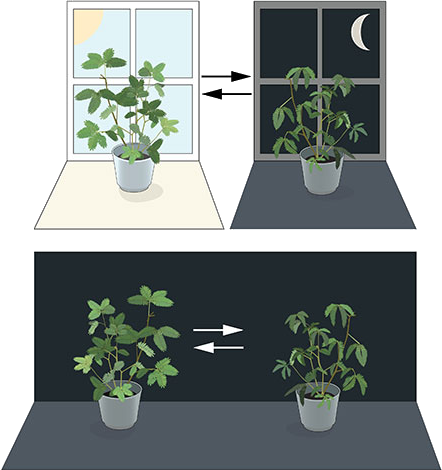
\includegraphics[width=0.6\linewidth,height=\textheight,keepaspectratio]{qmd/images/nobel-prize-outreach-ab-2017-figure-1.png}

\legend{Source: Reproduction from \textcite{nobelprizeoutreachab}.}

}

\end{figure}%

Science has already showed and described various biological rhythms.
These rhythms can occur at different levels, whether at a macro level,
such as the menstrual cycle, or even at a micro level, such as rhythms
expressed within cells \autocite{roenneberg2016}. Like many other
biological phenomena, these are complex systems present in all living
beings, i.e., systems with a large number of connected parts that
presents stable macroscopic patterns (emergences, in this case, the
rhythms) arising from local interactions or the collective behavior of
its parts, giving the system properties not attained by the aggregate
summation \autocite{epstein1999,holland2014}. It is understood today
that the endogeneity of rhythms has provided organisms with an
anticipatory capacity, allowing them to organize resources and
activities before they are needed \autocite{marques2003}.

Despite the endogenous nature of these rhythms, they can still be
regulated by the external environment. Signals (cues) from the
environment that occur cyclically in nature and have the ability to
regulate biological rhythmic expression are called zeitgebers (from the
German \emph{zeit}, meaning time, and \emph{geber}, meaning donor
\autocite{cambridgeuniversitypress}). These zeitgebers act as
synchronizers by entraining the phases of the rhythms
\autocite{khalsa2003,kuhlman2018}
(Figure~\ref{fig-chapter-2-kuhlman-2018-figure-2b}). Among the known
zeitgebers are, for example, meal timing and changes in environmental
temperature \autocite{aschoff1981,roenneberg2016}. However, the most
influential of them is the light-dark cycle (or, simply, light
exposure). It is understood that the day/night cycle, resulting from the
rotation of the Earth, has provided the vast majority of organisms with
an oscillatory system with a periodic duration of approximately 24 hours
\autocite{kuhlman2018,roenneberg2007}.

\begin{figure}[H]

\caption{\label{fig-chapter-2-kuhlman-2018-figure-2b}Illustration of a
circadian rhythm (output) whose phase is entrained in the presence of a
zeitgeber (input).}

\centering{

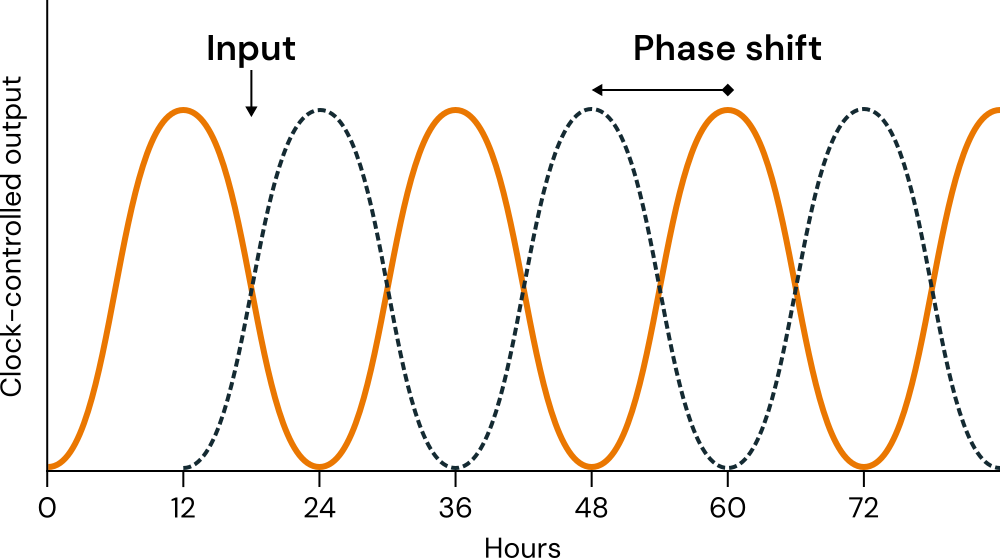
\includegraphics[width=0.85\linewidth,height=\textheight,keepaspectratio]{qmd/images/kuhlman-2018-figure-2b-adapted.png}

\legend{Source: Created by the author. Adapted from \textcite[Figure
2B]{kuhlman2018}.}

}

\end{figure}%

Naturally, the expression of this temporal organization varies from
organism to organism, even among members of the same species, whether
due to the different ways they are exposed to the environment or the
differences in the expression of endogenous rhythmicity, which, in turn,
results from gene expression \autocite{roenneberg2007a}. The interaction
between these two expressions, external and internal, of the environment
and genotype, generates a signature, an observable characteristic, which
is called a phenotype \autocite{frommlet2016}.

The various temporal characteristics of an organism can be linked to
different oscillatory periods. Among these are circadian phenotypes,
which refer to characteristics observed in rhythms with periods lasting
about a day \autocite{foster2005}. Another term used for these temporal
phenotypes, as the name suggest, is \emph{chronotype}
\autocite{ehret1974,pittendrigh1993}. This term is also often used to
differentiate phenotypes on a spectrum ranging from morningness to
eveningness \autocite{horne1976,roenneberg2019b}.

Sleep is a phenomenon that exhibits circadian expression. By observing
the sleep characteristics of individuals, it is possible to assess the
distribution of circadian phenotypes within a population, thereby
investigating their covariates and other relevant associations
\autocite{roenneberg2003}. This is because sleep regulation is
understood as the result of the interaction between two processes: a
homeostatic process (referred to as the \(\text{S}\) process), which is
sleep-dependent and accumulates with sleep deprivation; and a circadian
process (referred to as the \(\text{C}\) process), whose expression can
be influenced by zeitgebers, such as the light-dark cycle
(Figure~\ref{fig-chapter-2-borbely-1982-figure-4} illustrates these two
process) \autocite{borbely1982,borbely2016}. Considering that the
circadian rhythm (the \(\text{C}\) process) is present in sleep, its
characteristics can be estimated if the \(\text{S}\) process can be
controlled.

\begin{figure}[H]

\caption{\label{fig-chapter-2-borbely-1982-figure-4}Illustration of the
interaction between Process \(\text{S}\) (sleep-dependent process) and
Process \(\text{C}\) (circadian rhythm process) in sleep regulation.
\microskip \\ The figure depicts two scenarios: one with \(17\) hours of
wakefulness followed by \(7\) hours of sleep; and another, with sleep
deprivation, consisting of \(41\) hours of wakefulness followed by \(7\)
hours of sleep. The y-axis represents the level of each process. The
hatched areas indicate periods of sleep, along with the exponential
decline of Process \(\text{S}\).}

\centering{

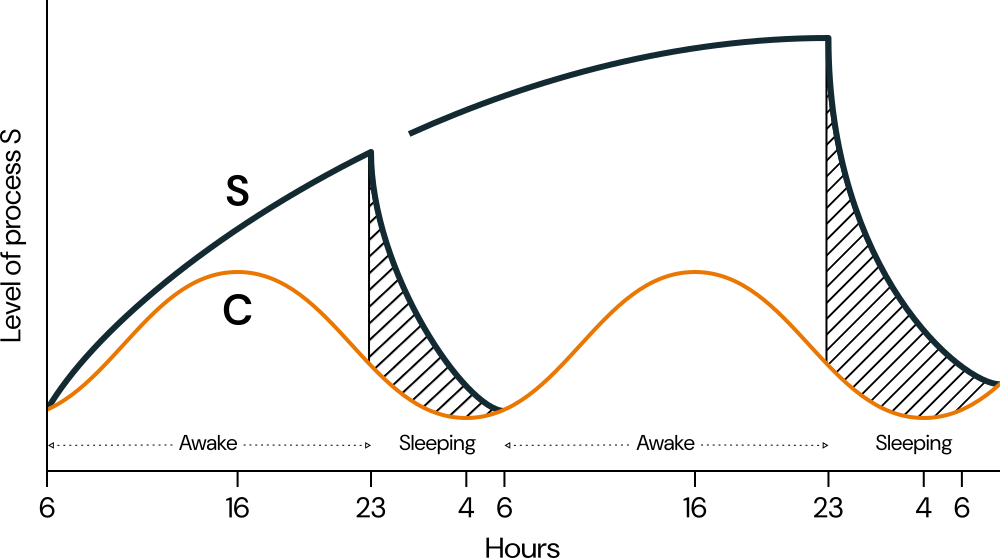
\includegraphics[width=0.85\linewidth,height=\textheight,keepaspectratio]{qmd/images/borbely-1982-figure-4-adapted.png}

\legend{Source: Created by the author. Adapted from \textcite[Figure 4,
lower part]{borbely1982}.}

}

\end{figure}%

Building on this idea, \textcite{roenneberg2003} developed the Munich
Chronotype Questionnaire (MCTQ) to measure the circadian phenotype
through sleep patterns. The MCTQ asks individuals about their sleep
habits, such as the times they go to bed and wake up on workdays and
work-free days. Based on this information, the MCTQ calculates the local
time of the midpoint of sleep on work-free days
(Figure~\ref{fig-chapter-2-mctq-variables}) and, if sleep deprivation is
detected on workdays, adjusts the measurement accordingly. This
midpoint, reflecting sleep without social obligations, is thought to
represent the unabridged expression of the circadian rhythm. Given its
basis in the two processes of sleep regulation, the MCTQ provides a good
proxy for measuring the circadian phenotype (or \(\text{C}\) process)
\autocite{leocadio-miguel2014}.

\begin{figure}[H]

\caption{\label{fig-chapter-2-mctq-variables}Variables of the Munich
ChronoType Questionnaire scale (a sleep log). In its standard version,
these variables are collected in the context of workdays and work-free
days. \microskip \\ BT = Local time of going to bed. SPrep = Local time
of preparing to sleep. SLat = Sleep latency \emph{or} time to fall
asleep after preparing to sleep. SO = Local time of sleep onset. SD =
Sleep duration. \textbf{MS} = Local time of mid-sleep. SE = Local time
of sleep. Alarm = A logical value indicating if the respondent uses an
alarm clock to wake up. SE = Local time of sleep end. SI = ``Sleep
inertia'' (despite the name, this variable represents the time the
respondent takes to get up after sleep end). GU = Local time of getting
out of bed. TBT = Total time in bed.}

\centering{

\pandocbounded{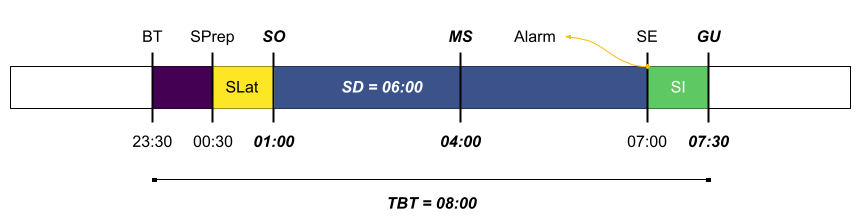
\includegraphics[keepaspectratio]{qmd/images/mctq-figure-1.png}}

\legend{Source: Created by the author.}

}

\end{figure}%

For this thesis, the MCTQ serves as the instrument for measuring
subjects' chronotypes (circadian phenotypes). The study uses a dataset
of \(65,824\) Brazilian respondents from an online survey conducted by
the author in 2017, which includes geographical data such as postal
codes. This data enables the examination of the potential association
between chronotype and geographic factors, particularly latitude and
longitude. The research ultimately seeks to determine whether latitude
plays a role in shaping chronotype, contributing to our understanding of
circadian rhythms in relation to geographic variables.

\bookmarksetup{startatroot}

\chapter{On the Latitude
Hypothesis}\label{sec-on-the-latitude-hypothesis}

The first mention of this hypothesis in English scientific literature
dates back to at least 1973, as noted by \textcite{bohlen1973}, with
earlier hints of the idea from Erhard Haus and Franz Halberg in 1970
\autocite[101]{haus1970}, building on discussions initiated by Jürgen
Aschoff \autocite{aschoff1969}. Since then, numerous studies have
explored this topic, yielding somewhat conflicting results (a systematic
review is provided by \textcite{randler2017}).

The hypothesis, also called \emph{environment hypothesis}, posits that
regions closer to the poles receive, on average, less annual sunlight
compared to regions near the equator
(Figure~\ref{fig-chapter-4-hut-2013-figure-1}). Consequently, regions
around latitude 0° are thought to have a stronger solar zeitgeber.
According to chronobiological theories, this stronger zeitgeber would
enhance the synchronization of circadian rhythms with the light-dark
cycle, resulting in lower variability and amplitude of circadian
phenotypes. This reduced influence of individual endogenous periods is
illustrated in
Figure~\ref{fig-chapter-4-roenneberg-2003-figure-7-f-adapted}.

In contrast, populations near the poles experience a weaker solar
zeitgeber, leading to greater variability and amplitude of circadian
phenotypes. This disparity translates into differences in chronotype:
equatorial populations tend to exhibit a morningness orientation, while
populations at higher and low latitudes tend toward eveningness
\autocite{bohlen1973,roenneberg2003}.

\begin{figure}[H]

\caption{\label{fig-chapter-4-hut-2013-figure-1}Annual changes in (a)
twilight duration, (b) daylight hours, and (c) temperature across
different latitudes. \microskip \\ Each color shows a specific latitude,
illustrating how these factors vary throughout the year.}

\centering{

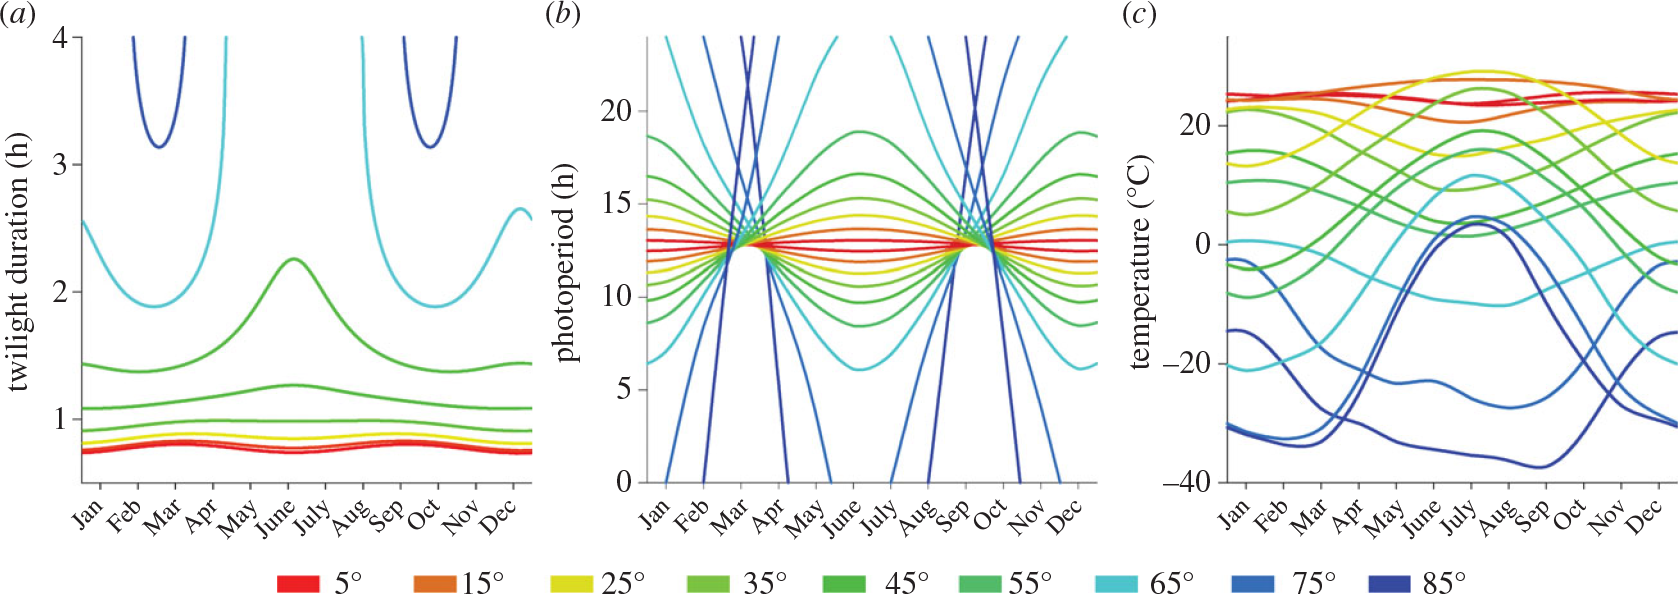
\includegraphics[width=1\linewidth,height=\textheight,keepaspectratio]{qmd/images/hut-2013-figure-1.png}

\legend{Source: Reproduction from \textcite{hut2013}.}

}

\end{figure}%

Some authors claim to found this association, but a closer look at the
data reveals that it is not as clear as it seems. For example,
\textcite{leocadio-miguel2017} found a significant association between
latitude and chronotype in a sample of \(12,884\) Brazilian
participants. However, the effect size was negligible, with latitude
explaining only about \(0.388\%\) of the variance in chronotype
(Figure~\ref{fig-chapter-4-leocadio-miguel-2017-figure-2}). Considering
the particular emphasis that the solar zeitgeber has on the entrainment
of biological rhythms (as demonstrated in many experiments), it would
not be reasonable to assume that the latitude hypothesis could be
supported without at least a non-negligible effect size.

\begin{figure}[H]

\caption{\label{fig-chapter-4-roenneberg-2003-figure-7-f-adapted}Different
chronotype distributions, influenced by strong and weak zeitgebers --
orange for strong (leptokurtic) and black for weak (platykurtic).
\microskip \\ An illustration of the effect hypothesized by the latitude
hypothesis.}

\centering{

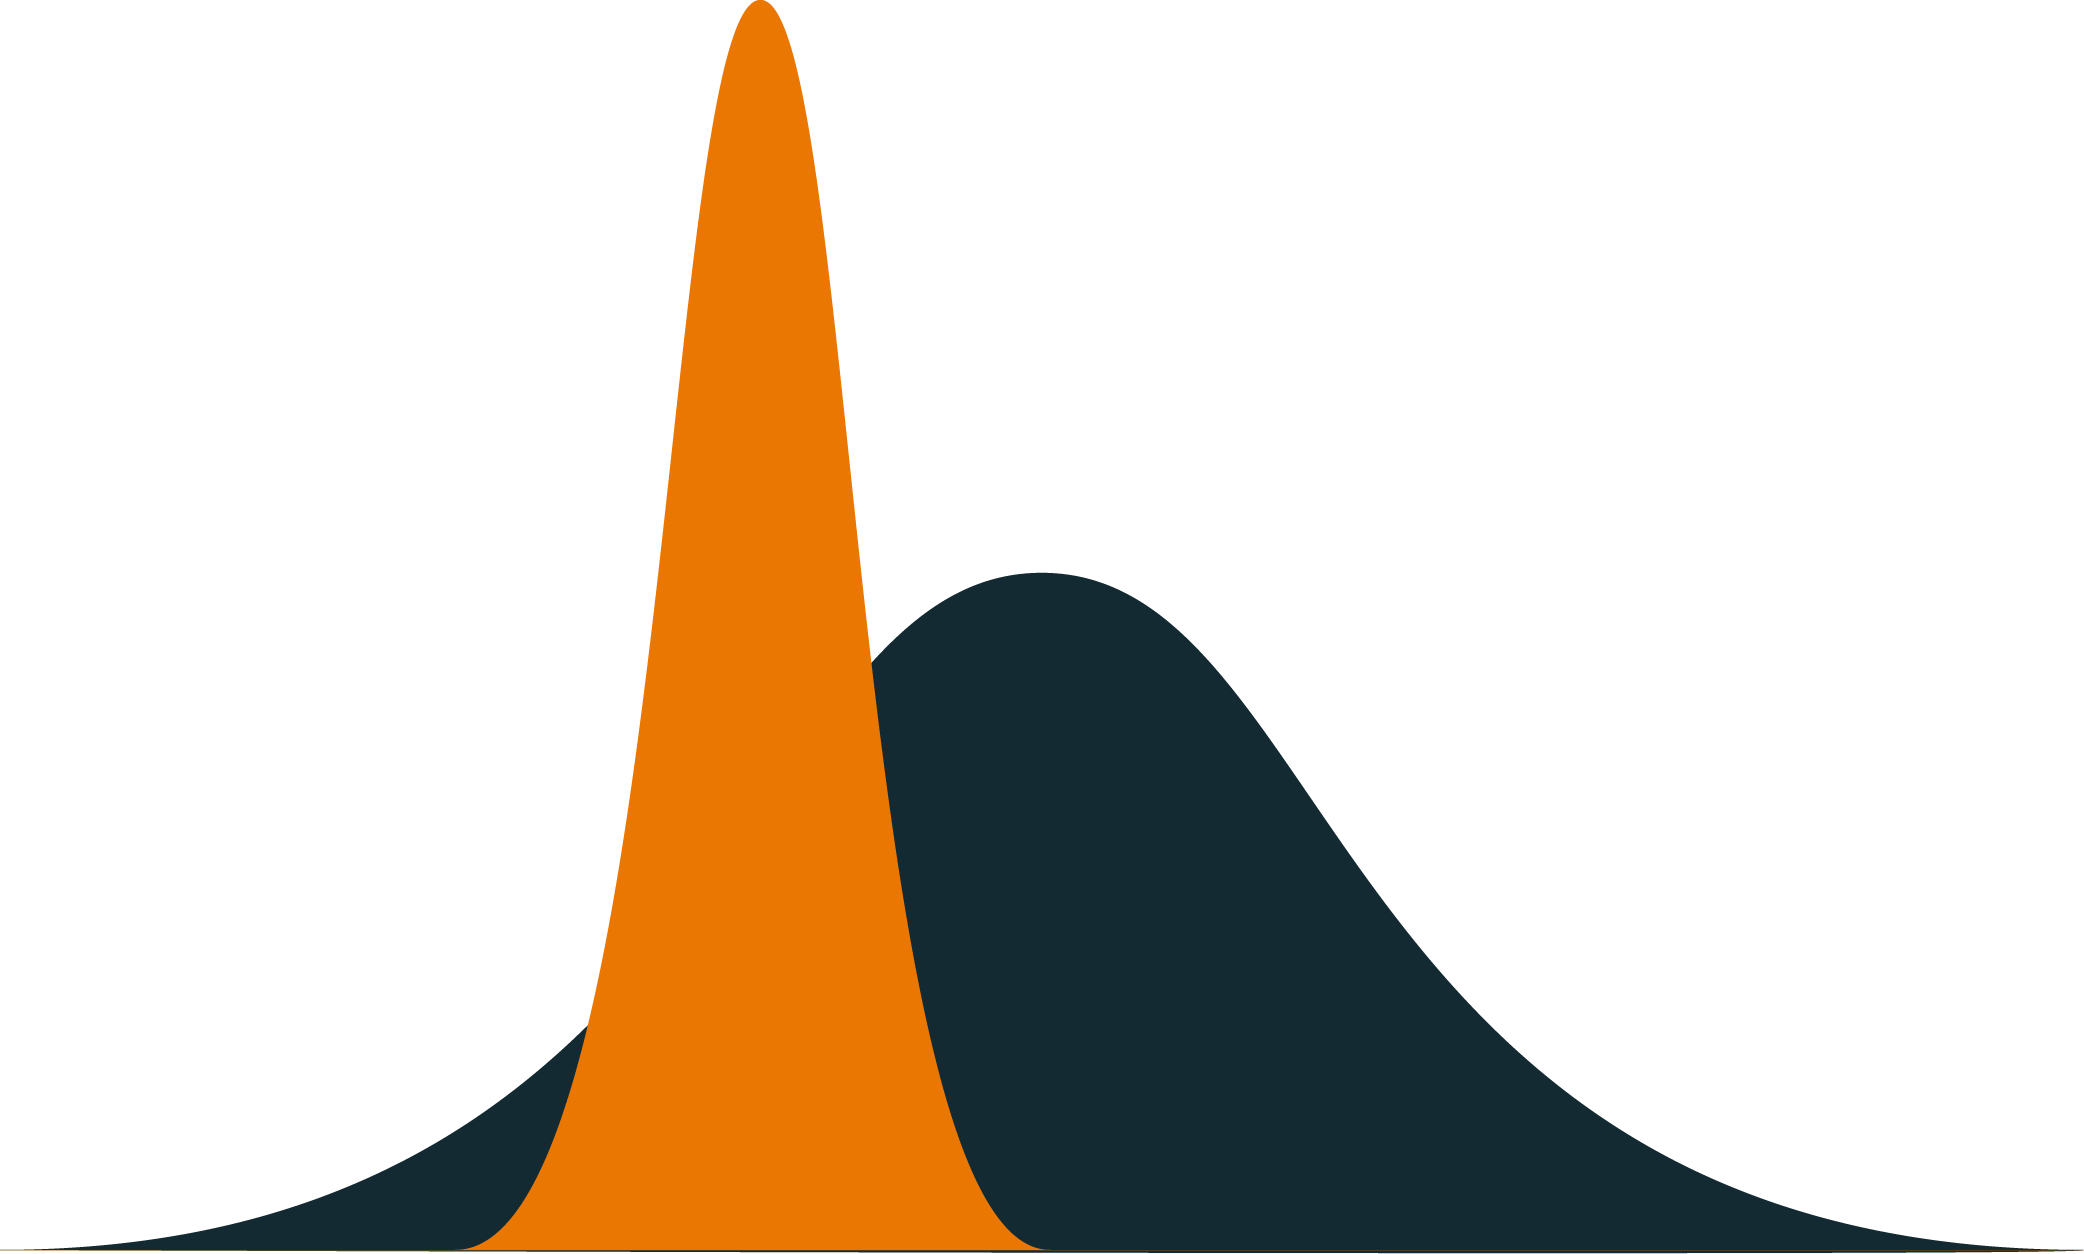
\includegraphics[width=0.75\linewidth,height=\textheight,keepaspectratio]{qmd/images/roenneberg-2003-figure-7-f-adapted.png}

\legend{Source: Created by the author. Adapted from \\ \textcite[Figure
7F]{roenneberg2003}.}

}

\end{figure}%

The findings of \textcite{leocadio-miguel2017} are not consistent with
the hypothesis that latitude is a strong predictor of chronotype, as the
reported effect size is too small to be considered practically
significant \autocite{cohen1988}. This highlights a common limitation of
studies relying on Null Hypothesis Significance Testing (NHST)
\autocite{perezgonzalez2015}. A p-value does not measure the effect
size; instead, it represents the conditional probability of observing
the data/test statistic (or something more extreme) assuming the null
hypothesis is true, thus quantifying the likelihood of a type I error
\autocite{cohen1994,wasserstein2016}.

\begin{figure}[H]

\caption{\label{fig-chapter-4-leocadio-miguel-2017-figure-2}Mean scores
(±SE) on the Horne \& Östberg (HO) chronotype scale \autocite{horne1976}
across a latitudinal gradient, along with the corresponding annual
average solar irradiation levels (W/m²). \microskip \\ The HO scale
comprises 19 items, with total scores ranging from 16 to 86; lower
scores indicate a stronger evening orientation, while higher scores
reflect a greater morning orientation. Notably, the y-axis exaggerates
the visual impact of the differences, as it represents a range of only
about 4.5 points, which may overstate the perceived significance of the
effect.}

\centering{

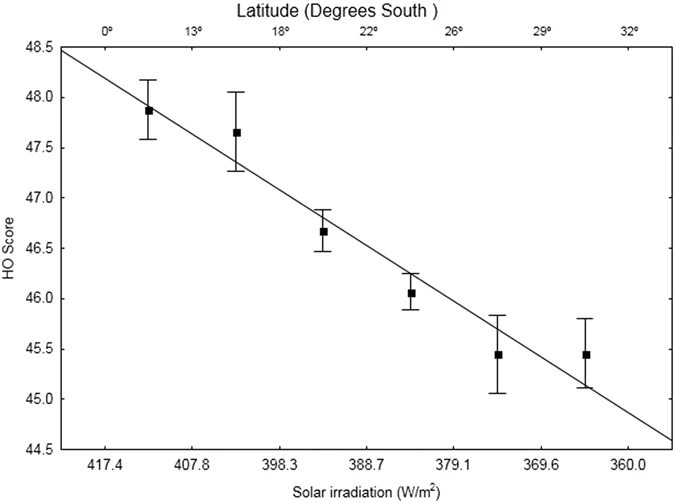
\includegraphics[width=0.85\linewidth,height=\textheight,keepaspectratio]{qmd/images/leocadio-miguel-2017-figure-2.png}

\legend{Source: Reproduction from \textcite{leocadio-miguel2017}.}

}

\end{figure}%

Several factors may invalidate this hypothesis, such as local clock time
and social constraints \autocite{skeldon2021}. To gain a more accurate
understanding of the mechanisms underlying chronotype expression, it
remains crucial to test this hypothesis in larger samples. This study
aims to address that gap.

In the following sections, the hypothesis will be tested using one of
the largest chronotype datasets, to the author's knowledge, with
geocoding information integrated for a comprehensive analysis. The
approach will adhere to sound statistical principles, incorporating a
minimum effect size in the alternative hypothesis, as originally
proposed by Neyman and Pearson data testing framework
\autocite{neyman1928,neyman1928a}.

\newpage

\null\vfill

\begingroup
\hyphenpenalty=100000
\noindent The following study was designed for publication in the journal \href{https://www.nature.com/srep/}{\textit{Scientific Reports}} (\href{https://jcr.clarivate.com/jcr}{IF 2023: 3.8/JCR} | \href{https://sucupira-legado.capes.gov.br/sucupira/}{CAPES: A1/2017-2020}) and structured in accordance with the journal's \href{https://www.nature.com/srep/author-instructions/submission-guidelines}{submission guidelines}.
\endgroup

\vspace{\hugeskipamount}

\bookmarksetup{startatroot}

\chapter{Is Latitude Associated with
Chronotype?}\label{sec-latitude-hypothesis-article}

\section{Abstract}\label{abstract}

\noindent \textbf{Chronotypes are temporal phenotypes that reflect our
internal temporal organization, a product of evolutionary pressures
enabling organisms to anticipate events. These intrinsic rhythms are
modulated by zeitgebers --- environmental stimuli that entrain these
biological oscillations, with light exposure being the primary
mechanism. Given light's role in these systems, previous research
hypothesized that latitude might significantly influence chronotypes,
suggesting that populations near the equator would exhibit more
morning-leaning characteristics due to more consistent light-dark
cycles, while populations near the poles might display more
evening-leaning tendencies with a potentially freer expression of
intrinsic rhythms. To test this hypothesis, we analyzed chronotype data
from a large sample of \(65,824\) subjects across diverse latitudes in
Brazil. Our results revealed that latitude show only negligible effect
sizes on chronotype, indicating that the entrainment phenomenon is far
more complex than previously conceived. These findings challenge
simplified environmental models of biological timing and underscore the
need for more nuanced investigations into the mechanisms underlying
temporal phenotypes, opening new avenues for understanding the intricate
relationship between environmental cues and individual circadian
rhythms.}

\section{Introduction}\label{introduction}

Humans exhibit a variety of observable traits, such as eye or hair
color, which are referred to as phenotypes. These phenotypes also
manifest in the way our bodies function.

A chronotype is a temporal phenotype
\autocite{ehret1974,pittendrigh1993}, typically used to refer to
endogenous circadian rhythms --- biological rhythms with periods close
to 24 hours. Chronobiology, the science that studies biological rhythms,
suggests that the evolution of these internal oscillators is closely
linked to our environment, particularly the day-night cycle. This cycle,
alongside human evolution, created environmental pressures that led to
the development of temporal organization within organisms
\autocite{aschoff1989,paranjpe2005}. Such temporal organization allowed
organisms to predict events and better manage their needs, such as
storing food for winter.

For a temporal system to be useful, it must be capable of adapting to
environmental changes. Environmental signals capable of regulating
biological rhythms are known as zeitgebers (from the German \emph{zeit},
meaning time, and \emph{geber}, meaning donor
\autocite{cambridgeuniversitypress}). These zeitgebers provide inputs
that can shift and synchronize biological rhythms. This process is
called entrainment \autocite{roenneberg2003a,roenneberg2010}.

The primary zeitgeber influencing biological rhythms is light,
particularly sunlight \autocite{aschoff1972}. Given its significant role
in entraining the biological clock, several studies have hypothesized
that the latitudinal shift of the sun, due to the Earth's axial tilt,
might lead to different temporal traits in populations near the equator
compared to those closer to the poles
\autocite{bohlen1973,pittendrigh1991,roenneberg2003,randler2008,hut2013,leocadio-miguel2017,randler2017}.
This is based on the idea that populations at low or higher latitudes
experience greater fluctuations in sunlight and a weaker overall solar
zeitgeber. This concept is known as the latitude hypothesis, or the
environmental hypothesis of circadian rhythm regulation.

Recent efforts to test the latitude hypothesis in humans have largely
been unsuccessful in identifying a significant effect related to
latitude. Many of these studies used secondary data or small sample
sizes. A notable attempt was made by Leocadio-Miguel et al.
\autocite*{leocadio-miguel2017}, who measured the chronotype of
\(12,884\) Brazilian subjects across a wide latitudinal range using the
Morningness--Eveningness Questionnaire (MEQ). Their findings showed a
negligible effect size. One possible explanation is that the MEQ
measures psychological traits rather than the biological states of
circadian rhythms themselves \autocite{roenneberg2019}, meaning it might
not be the most suitable tool for testing the hypothesis
\autocite{leocadio-miguel2014}.

This study presents a novel attempt to test the latitude hypothesis,
using a biological approach through the Munich ChronoType Questionnaire
(MCTQ) \autocite{roenneberg2003}. In addition, it utilizes the largest
dataset on chronotype in a single country, as far as the existing
literature suggests, comprising \(65,824\) respondents, all living
within the same timezone in Brazil and completing the survey within a
one-week window
(Figure~\ref{fig-chapter-5-sample-geographical-distribution}).

\begin{figure}[H]

\caption{\label{fig-chapter-5-sample-geographical-distribution}Geographical
distribution of the sample used in the analysis: (\(n = 65,824\)).
\microskip \\ Each point represents a municipality, with its size
proportional to the number of participants and its color indicating
participant density. The sample includes Brazilian individuals aged 18
or older, residing in the UTC-3 timezone, who completed the survey
between October 15 and 21, 2017. The size and color scale are
logarithmic (\(\log_{10}\)).}

\centering{

\pandocbounded{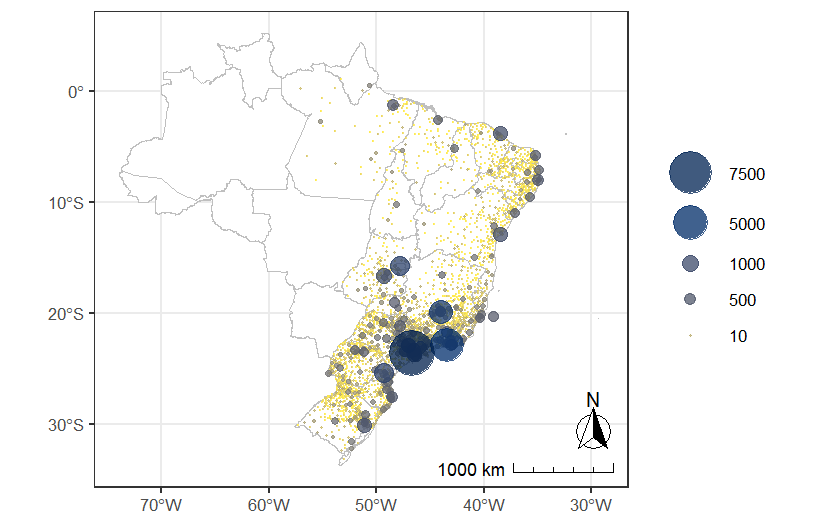
\includegraphics[keepaspectratio]{qmd/chapter-5_files/figure-pdf/unnamed-chunk-6-1.png}}

\legend{Source: Created by the author.}

}

\end{figure}%

\section{Results}\label{results}

The local time of the sleep-corrected midpoint between sleep onset and
sleep end on work-free days (MSFsc), which serves as the MCTQ proxy for
measuring chronotype, had an overall mean of \(\text{04:28:41}\) and a
standard deviation of \(\text{01:26:13}\). The distribution is shown in
Figure~\ref{fig-chapter-5-chronotype-distribution}.

This represents the midsleep point for Brazilian subjects with an
intermediate or average chronotype. Considering the 7--9 hours of sleep
recommended for healthy adults by the American Academy of Sleep Medicine
(AASM) \autocite{watson2015}, one could imagine that this average
individual, in the absence of social restrains, would typically wake up
at approximately \(\text{08:28:41}\).

\begin{figure}[H]

\caption{\label{fig-chapter-5-chronotype-distribution}Distribution of
the local time for the sleep-corrected midpoint between sleep onset and
sleep end on work-free days (MSF\textsubscript{sc}), a proxy for
chronotype. \microskip \\ Chronotypes are categorized into quantiles,
ranging from extremely early (\(0 |- 0.11\)) to extremely late
(\(0.88 - 1\)).}

\centering{

\pandocbounded{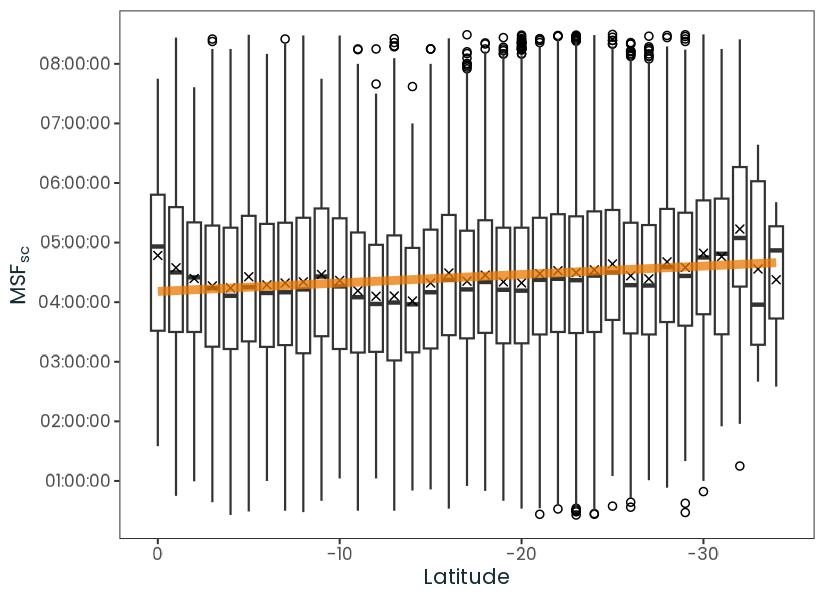
\includegraphics[keepaspectratio]{qmd/chapter-5_files/figure-pdf/unnamed-chunk-7-1.png}}

\legend{Source: Created by the author. Based on data visualization found
in \\ \textcite{roenneberg2019b}.}

}

\end{figure}%

The study hypothesis was tested using nested multiple linear
regressions. The core idea of nested models is to evaluate the effect of
including one or more predictors on the model's variance explanation
(\(\text{R}^2\)) \autocite{maxwell2018}. This is achieved by comparing a
restricted model with a full model. Cell weights, based on sex, age
group, and state of residence, were used to account for sample
imbalances.

Two tests were conducted, both using the same restricted model, which
included age, sex, longitude, and the monthly Global Horizontal
Irradiance (GHI) average at the time of questionnaire completion as
predictors (\(\text{Adjusted R}^{2} = 0.085110\);
\(\text{F}(4, 65818) = 1530\), \(\text{p-value} < 2e-16\)). The first
full model (\textbf{A}) added annual GHI average and daylight duration
for the nearest March equinox, as well as the June and December
solstices, as proxies for latitude, following
\textcite{leocadio-miguel2017} methods
(\(\text{Adjusted R}^{2} = 0.087921\); \(\text{F}(8, 65814) = 794\),
\(\text{p-value} < 2e-16\)). The second full model (\textbf{B}) added
only latitude as a predictor (\(\text{Adjusted R}^{2} = 0.085614\);
\(\text{F}(5, 65817) = 1230\), \(\text{p-value} < 2e-16\)). All
coefficients were significantly different from zero
(\(\text{p-value} = 2e-16\)). Assumption checking and residual
diagnostics primarily relied on visual inspection, as objective
assumption tests (e.g., Anderson--Darling) are not advisable for large
samples \autocite{shatz2024}. All validity assumptions were met, and no
serious multicollinearity was found among the predictor variables.

Sunrise times for the nearest March and September equinoxes, as well as
the June and December solstices, were excluded due to high
multicollinearity. Daylight duration for the September equinox was
excluded for its multicollinearity with daylight duration during the
March equinox.

An \(\text{F}\) test for nested models revealed a significant reduction
in the residual sum of squares (\textbf{A}
\(\text{F}(4, 65814) = 51.71\), \(\text{p-value} < 2e-16\); \textbf{B}
\(\text{F}(1, 65817) = 37.325\), \(\text{p-value} < 1e-9\)). However,
when estimating Cohen's \(f^2\) effect size, the results were negligible
\autocite{cohen1992} (\textbf{A} \(f^{2} = 0.012137120\); \textbf{B}
\(f^{2} = 0.009523916\)).

\section{Discussion}\label{discussion}

It is important to emphasize that assuming a causal and linear
relationship between latitude and chronotype is an \emph{a priori}
hypothesis. The objective of this study is to test and potentially
falsify this hypothesis.

The results indicate that, despite a broad latitudinal spectrum and a
large, well-aligned sample, the latitude effect on chronotype does not
manifest in a meaningful way. Several studies have suggested a potential
effect of latitude on chronotype, but, at present, no empirical evidence
supports this claim in humans. These findings align with those of
\textcite{leocadio-miguel2017}, who observed a similar effect size
(Cohen's \(f^2 = 0.004143174\)). However, the earlier study did not
incorporate a minimum effect size criterion, which led to misleading
conclusions. The small and inconsistent size of the latitude effect can
be seen in Figure~\ref{fig-chapter-5-chronotype-latitude-series}.
Figure~\ref{fig-chapter-5-chronotype-geographical-distribution} shows
the distribution of chronotypes by the mean for each Brazilian state.

\begin{figure}[H]

\caption{\label{fig-chapter-5-chronotype-latitude-series}Boxplots of
mean MSF\textsubscript{sc} values aggregated by 1° latitude intervals,
illustrating the relationship between latitude and chronotype.
\microskip \\ MSF\textsubscript{sc} represents the local time of the
sleep-corrected midpoint between sleep onset and sleep end on work-free
days, a proxy for chronotype. Higher MSF\textsubscript{sc} values
indicate later chronotypes. The × symbol points to the mean. The orange
line represents a linear regression. The differences in mean/median
values across latitudes are minimal relative to the Munich ChronoType
Questionnaire (MCTQ) scale.}

\centering{

\pandocbounded{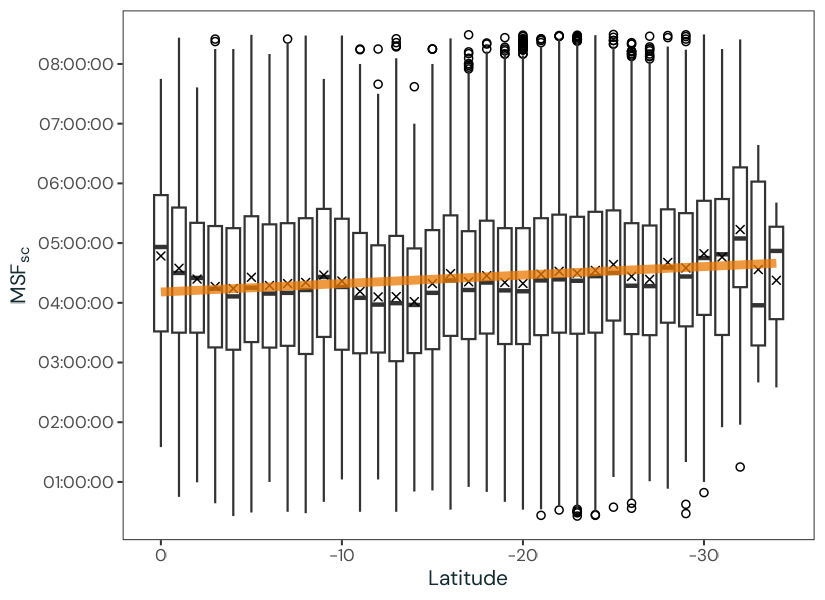
\includegraphics[keepaspectratio]{qmd/chapter-5_files/figure-pdf/unnamed-chunk-8-1.png}}

\legend{Source: Created by the author.}

}

\end{figure}%

The absence of a clear relationship between latitude and chronotype can
be attributed to multiple factors. As Jürgen Aschoff might have put it,
this may reflect a lack of ``ecological significance''
\autocite{aschoff1972}. Even if latitude does influence circadian
rhythms, the effect could be too minor to detect or might be
overshadowed by other, more prominent factors like social behaviors,
work hours, or the widespread use of artificial lighting
\autocite{bohlen1973}. Furthermore, the variations in sunlight exposure
between latitudes may not be substantial enough to meaningfully impact
the circadian system, which is highly responsive to light. Since even
small fluctuations in light exposure can lead to measurable
physiological changes, it suggests that latitude alone may not be a
decisive factor in determining chronotype.

\begin{figure}[H]

\caption{\label{fig-chapter-5-chronotype-geographical-distribution}Geographical
distribution of mean mid-sleep on free days sleep-corrected
(MSF\textasciitilde sc) values by Brazilian state, illustrating how
chronotype varies with latitude in Brazil. \microskip \\
MSF\textsubscript{sc} is a proxy for chronotype, representing the
midpoint of sleep on work-free days, adjusted for sleep debt. Higher
MSF\textsubscript{sc} values correspond to later chronotypes. The color
scale was not transformed and it has as limits the first and third
quartile (interquartile range). Differences in mean
MSF\textsubscript{sc} values across states are small and fall within a
narrow range relative to the scale of the Munich ChronoType
Questionnaire (MCTQ), limiting the significance of these variations.}

\centering{

\pandocbounded{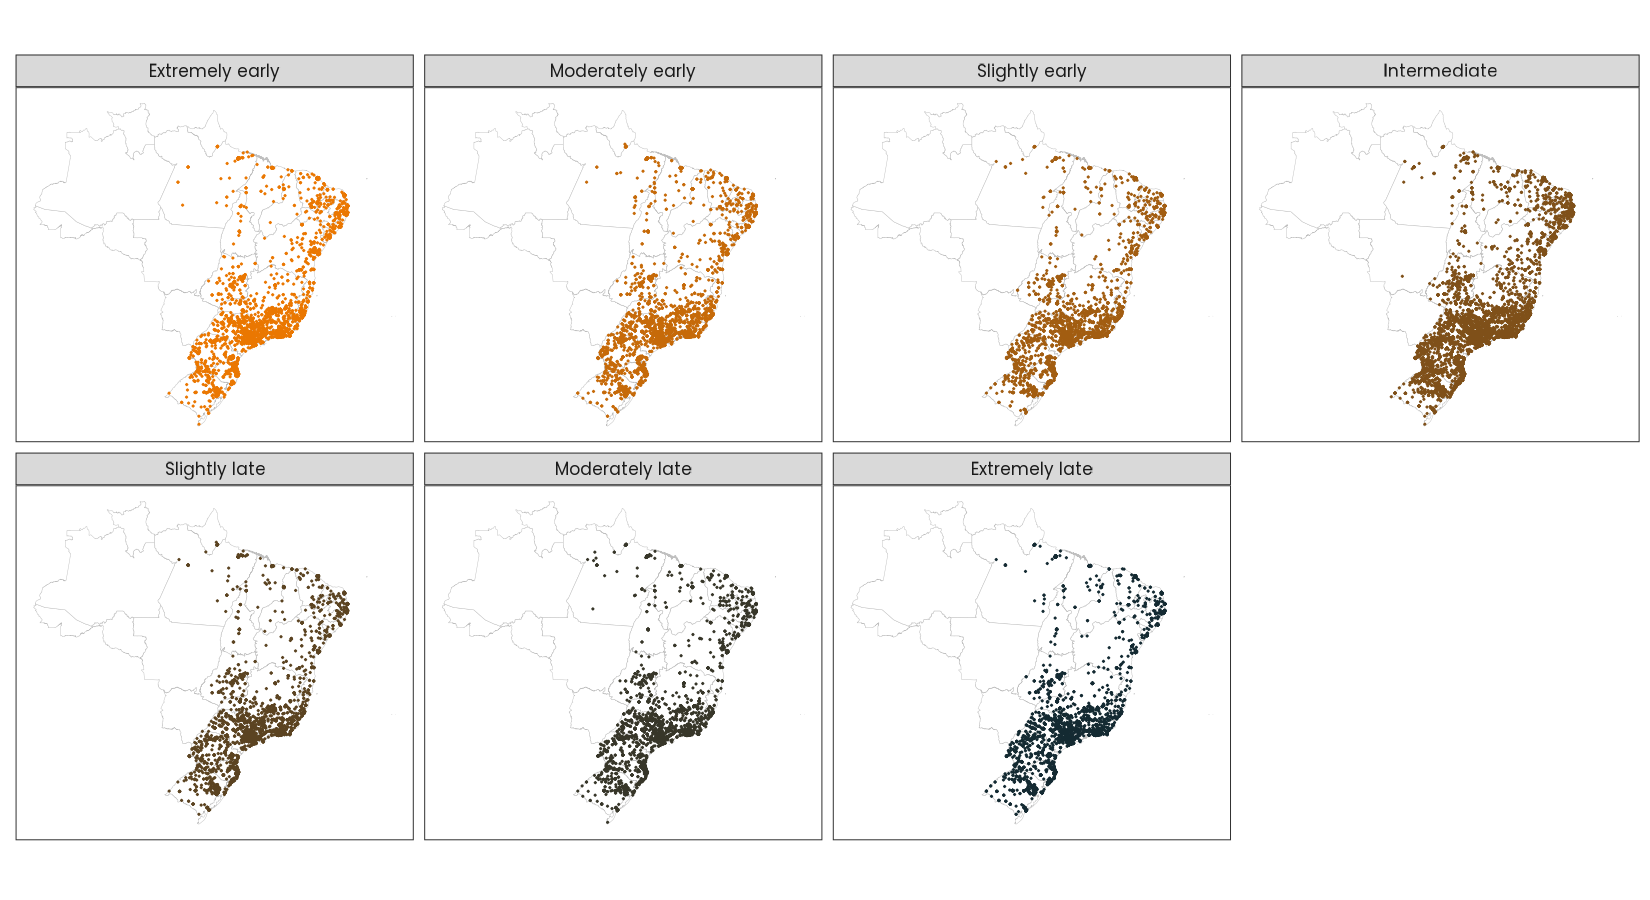
\includegraphics[keepaspectratio]{qmd/chapter-5_files/figure-pdf/unnamed-chunk-9-1.png}}

\legend{Source: Created by the author.}

}

\end{figure}%

This study points to a more intricate relationship between latitude and
the circadian system than originally expected. In human populations, the
perceived link between these variables might have been influenced by
statistical overconfidence, driven by routine reliance on Null
Hypothesis Significance Testing (NHST) and the tendency to confirm
preconceived ideas, rather than a rigorous and unbiased examination of
the data.

\section{Methods}\label{methods}

\subsection{Measurement Instrument}\label{measurement-instrument}

Chronotypes were assessed using a sleep log based on the core version of
the standard Munich ChronoType Questionnaire (MCTQ)
\autocite{roenneberg2003}, a well-validated and widely applied
self-report tool for measuring sleep-wake cycles and chronotypes
\autocite{roenneberg2019}. The MCTQ captures chronotype as a biological
circadian phenotype, determined by the sleep-corrected midpoint of sleep
(MS) (Figure~\ref{fig-chapter-5-mctq-variables}) on work-free days
(MSF), accounting for any potential sleep compensation due to sleep
deficits (sc = sleep correction) on workdays (MSF\textsubscript{sc})
\autocite{roenneberg2012}.

\begin{figure}[H]

\caption{\label{fig-chapter-5-mctq-variables}Variables of the Munich
ChronoType Questionnaire scale (a sleep log). In its standard version,
these variables are collected in the context of workdays and work-free
days.\microskip \\ BT = Local time of going to bed. SPrep = Local time
of preparing to sleep. SLat = Sleep latency \emph{or} time to fall
asleep after preparing to sleep. SO = Local time of sleep onset. SD =
Sleep duration. MS = Local time of mid-sleep. SE = Local time of sleep.
Alarm = A logical value indicating if the respondent uses an alarm clock
to wake up. SE = Local time of sleep end. SI = ``Sleep inertia''
(despite the name, this variable represents the time the respondent
takes to get up after sleep end). GU = Local time of getting out of bed.
TBT = Total time in bed.}

\centering{

\pandocbounded{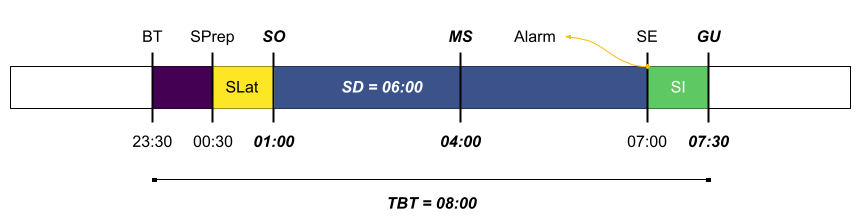
\includegraphics[keepaspectratio]{qmd/images/mctq-figure-1.png}}

\legend{Source: Created by the author.}

}

\end{figure}%

Participants completed an online questionnaire, which included the sleep
log as well as sociodemographic (e.g., age, sex), geographic (e.g., full
residential address), anthropometric (e.g., weight, height), and data on
work or study routines. A sample version of the questionnaire, stored
independently by the \href{https://archive.org/}{Internet Archive}
organization can be viewed at
\url{https://web.archive.org/web/20171018043514/each.usp.br/gipso/mctq}.

\subsection{Sample}\label{sample}

The dataset used for analysis was made up of \(65,824\) Brazilian
individuals aged 18 or older, residing in the UTC-3 timezone, who
completed the survey between October 15 and 21, 2017.

The unfiltered valid sample comprises \(115,166\) participants from all
Brazilian states, while the raw sample is composed of \(120,265\)
individuals. The majority of the sample data was obtained in 2017 from
October 15th to 21st by \href{https://globoplay.globo.com/v/6219513/}{a
broadcast} of the online questionnaire on a popular Brazil's Sunday TV
show with national reach \autocite{redeglobo2017}. This amount of data
collected in such a short time gave the sample a population
cross-sectional characteristic.

Based on 2017 data from the Brazilian Institute of Geography and
Statistics's (\href{https://www.ibge.gov.br/}{IBGE}) Continuous National
Household Sample Survey
(\href{https://www.ibge.gov.br/estatisticas/sociais/trabalho/17270-pnad-continua.html}{PNAD
Contínua}) \autocite{ibgee}, Brazil had \(51.919\%\) of females and
\(48.081\%\) of males with an age equal to or greater than 18 years old.
The sample is skewed for female subjects, with \(66.433\%\) of females
and \(33.567\%\) of male subjects. To balance the sample, a weighting
procedure was applied to the data. The weights were calculated by cell
weighting, using the sex, age group and Brazil's state as reference.

A survey conducted in 2019 by the Brazilian Institute of Geography and
Statistics (IBGE) \autocite*{ibge2021} found that \(82.17\%\) of
Brazilian households had access to an internet connection. Therefore,
this sample is likely to have a good representation of Brazil's
population.

The sample latitudinal range was \(33.85026\) decimal degrees
(\(\text{Min.} = -33.522\); \(\text{Max.} = 0.329\)) with a longitudinal
span of \(22.741\) decimal degrees (\(\text{Min.} = -57.553\);
\(\text{Max.} = -34.812\)). For comparison, Brazil has a latitudinal
range of \(39.023\) decimal degrees (\(\text{Min.} = -33.751\);
\(\text{Max.} = 5.272\)) and a longitudinal span of \(45.155\) decimal
degrees (\(\text{Min.} = -73.990\); \(\text{Max.} = -28.836\)).

More information about the sample can be found in the supplementary
materials.

\subsection{Data Wrangling}\label{data-wrangling}

Data wrangling and analysis followed the data science program proposed
by Hadley Wickham and Garrett Grolemund \autocite{wickham2016}. All
processes were made with the help of the R programming language
\autocite{rcoreteam}, RStudio IDE \autocite{positteam}, and several R
packages. The \href{https://www.tidyverse.org/}{tidyverse} and
\href{https://ropensci.org/}{rOpenSci} peer-reviewed package ecosystem
and other R packages adherents of the tidy tools manifesto
\autocite{wickham2023} were prioritized. The MCTQ data was analyzed
using the \texttt{mctq} rOpenSci peer-reviewed package
\autocite{vartaniana}. All processes were made in order to provide
result reproducibility and to be in accordance with the FAIR principles
\autocite{wilkinson2016}.

\subsection{Hypothesis Test}\label{hypothesis-test}

The study hypothesis was tested using nested models general linear
models of multiple linear regressions. It was schematized as follows.

\begin{itemize}
\item
  \textbf{Null hypothesis} (\(\text{H}_{0}\)): Adding \emph{latitude}
  does not meaningfully improve the model's fit, indicating that the
  change in adjusted \(\text{R}^{2}\) is negligible or the F-test is not
  significant (considering a type I error probability (\(\alpha\)) of
  \(0.05\)).
\item
  \textbf{Alternative Hypothesis} (\(\text{H}_{a}\)): Adding
  \emph{latitude} meaningfully improves the model's fit, indicating that
  the change in adjusted \(\text{R}^{2}\) is greater than the Minimum
  Effect Size (MES), and the F-test is significant (considering a type I
  error probability (\(\alpha\)) of \(0.05\)).
\end{itemize}

\[
\begin{cases}
\text{H}_{0}: \Delta \ \text{Adjusted} \ \text{R}^{2} \leq \text{MES} \quad \text{or} \quad \text{F-test is not significant} \ (\alpha \geq 0.05) \\
\text{H}_{a}: \Delta \ \text{Adjusted} \ \text{R}^{2} > \text{MES} \quad \text{and} \quad \text{F-test is significant} \ (\alpha < 0.05)
\end{cases}
\]

\medskip

Where:

\[
\Delta \ \text{Adjusted} \ \text{R}^{2} = \text{Adjusted} \ \text{R}^{2}_{f} - \text{Adjusted} \ \text{R}^{2}_{r}
\]

\medskip

A MES must always be used in any data testing. The effect-size was
present in the original Neyman and Pearson framework
\autocite{neyman1928,neyman1928a}, but unfortunately this practice fade
away with the use of p-values, one of the many issues that came with the
Null Hypothesis Significance Testing (NHST)
\autocite{perezgonzalez2015}. While p-values are estimates of type 1
error (in Neyman--Pearson's approaches, or like-approaches), that's not
the main thing we are interested while doing a hypothesis test, what is
really being test is the effect size (i.e., a practical significance).
Another major issue to only relying on p-values is that the estimated
p-value tends to decrease when the sample size is increased, hence,
focusing just on p-values with large sample sizes results in the
rejection of the null hypothesis, making it not meaningful in this
specific situation \autocite{lin2013,mariscal2021}.

Considering the particular emphasis that the solar zeitgeber has on the
entrainment of biological rhythms (as demonstrated in many experiments),
it would not be reasonable to assume that the latitude hypothesis could
be supported without at least a non-negligible effect size. With this in
mind, this analysis used Cohen's \(f^{2}\) threshold for
small/negligible effects, the Minimum Effect Size (MES) is defined as
0.02 \autocites[413]{cohen1988}[157]{cohen1992}. For comparison, Cohen's
threshold for medium effects is \(0.15\), and for large effects is
\(0.35\).

Knowing Cohen's \(f^2\), is possible to calculated the equivalent
\(\text{R}^{2}\):

\[
0.02 = \cfrac{\text{R}^{2}}{1 - \text{R}^{2}} \quad \text{or} \quad \text{R}^{2} = \cfrac{0.02}{1.02} \eqsim 0.01960784
\]

\medskip

In other words, the latitude must explain at least \(1.960784\%\) of the
variance in the dependent variable to be considered non-negligible. This
is the Minimum Effect Size (MES) for this analysis.

In summary, the decision rule for the hypothesis test is as follows:

\begin{itemize}
\tightlist
\item
  \textbf{Reject} \(\text{H}_{0}\) \textbf{if both}:

  \begin{itemize}
  \tightlist
  \item
    The F-test is significant
  \item
    \(\Delta \ \text{Adjusted} \ \text{R}^{2} > 0.01960784\)
  \end{itemize}
\item
  \textbf{Fail to reject} \(\text{H}_{0}\) \textbf{if either}:

  \begin{itemize}
  \tightlist
  \item
    The F-test is not significant
  \item
    \(\Delta \ \text{Adjusted} \ \text{R}^{2} \leq 0.01960784\)
  \end{itemize}
\end{itemize}

As usual, the significance level (\(\alpha\)) was set at \(0.05\),
allowing a 5\% chance of a Type I error.

A power analysis was performed to determine the necessary sample size
for detecting the MES effect. The results indicate that at least
\(1,895\) observations per variable were required to achieve a power of
\(0.99\) (\(1 - \beta\)) and a significance level (\(\alpha\)) of
\(0.01\). The dataset contains \(65,824\) observations, which exceeds
this requirement.

\subsection{Data Availability}\label{data-availability}

Some restrictions apply to the availability of the main research data,
which contain personal and sensitive information. As a result, this data
cannot be publicly shared. Data are, however, available from the author
upon reasonable request.

Unrestricted data can be access on the research compendium via
\href{https://osf.io/}{The Open Science Framework} at the following
link: \url{https://doi.org/10.17605/OSF.IO/YGKTS}.

\subsection{Code Availability}\label{code-availability}

All analyses are fully reproducible and were conducted using the
\href{https://www.r-project.org/}{R programming language} alongside the
\href{https://quarto.org/}{Quarto} publishing system. The
\href{https://rstudio.github.io/renv/}{\texttt{renv}} package was used
to ensure that the R environment used can be restored (see
\texttt{renv.lock}).

The code repository is available on GitHub at
\url{https://github.com/danielvartan/mastersthesis}, and the research
compendium can be accessed via \href{https://osf.io/}{The Open Science
Framework} at the following link:
\url{https://doi.org/10.17605/OSF.IO/YGKTS}.

\section{Acknowledgments}\label{acknowledgments}

This study was financed in part by the Coordenação de Aperfeiçoamento de
Pessoal de Nível Superior - Brasil
(\href{https://www.gov.br/capes/}{CAPES}) - Finance Code 001, Grant
number 88887.703720/2022-00.

\section{Ethics Declarations}\label{ethics-declarations}

The author declares that the study was carried out without any
commercial or financial connections that could be seen as a possible
competing interest.

\section{Additional Information}\label{additional-information}

See the supplementary material for more information.

Correspondence can be sent to Daniel Vartanian
(\href{mailto:danvartan@gmail.com}{\nolinkurl{danvartan@gmail.com}}).

\section{Rights and Permissions}\label{rights-and-permissions}

This article is released under the
\href{http://creativecommons.org/licenses/by/4.0/}{Creative Commons
Attribution 4.0 International License}, which permits use, sharing,
adaptation, distribution, and reproduction in any medium or format, as
long as be given appropriate credit to the original author and the
source, provide a link to the Creative Commons license, and indicate if
changes were made.

\bookmarksetup{startatroot}

\chapter{Conclusion}\label{sec-conclusion}

According to Popper, the aim of science is to provide ``satisfactory
explanations of whatever strikes us as being in need of explanation''
\autocite[193]{popper1979}. This study, using what is arguably the
largest dataset on chronotype collected within a single time
zone---balanced to reflect population proportions at the time of data
collection---found no support for the latitude hypothesis (Cohen's
\(f^2 = 0.0121371\)). This result contributes meaningful evidence to the
understanding of circadian rhythm regulation, offering a clear and
satisfactory answer to the central research question of this thesis:
``Is latitude associated with chronotype?''. The answer is \textbf{No}.

These findings are consistent with those of
\textcite{leocadio-miguel2017}, who reported a similar effect size
(Cohen's \(f^2 = 0.004143174\)). However, the earlier study did not
apply a minimum effect size criterion, leading to a misleading
conclusion.

Several factors could explain the lack of an association between
latitude and chronotype ― or, as Jürgen Aschoff might have phrased it,
the absence of ``ecological significance'' \autocite{aschoff1972}. For
instance, if latitude does affect the circadian system, the effect may
be too small to detect or could be overshadowed by other influences,
such as social habits, work schedules, or the use of artificial light
\autocite{bohlen1973,skeldon2021}. Additionally, the difference in solar
exposure across latitudes may be insufficient to produce a meaningful
effect on the circadian system, which is highly sensitive to light. Even
minor variations in light exposure can yield significant physiological
responses, suggesting that latitude alone may not be a strong predictor
of chronotype.

These results suggest that the relationship between latitude and the
circadian system is far more complex than anticipated. In human
contexts, the perception of such an effect may have arisen from
statistical misinterpretations, driven by ritualistic reliance on Null
Hypothesis Significance Testing (NHST) and confirmation bias, rather
than a critical evaluation of the data.

\section{Limitations}\label{limitations}

While this study provides valuable insights, it is essential to
acknowledge certain limitations that may influence the interpretation of
the findings. First, the data collection occurred predominantly during a
single week in spring, as summer approached, which limited the
photoperiod variability between regions. A better approach would involve
data collection across different seasons, particularly during winter,
when photoperiod differences are more pronounced between equatorial and
polar regions.

Additionally, the use of the Munich Chronotype Questionnaire (MCTQ),
while a validated instrument, introduces the potential for recall and
social desirability biases inherent to self-reported measures. However,
the large sample size likely mitigates these biases, as predicted by the
law of large numbers \autocite[352]{degroot2012}. Furthermore, at the
time of data collection, the MCTQ had not yet been officially validated
in Portuguese (this was only introduced in 2020 by
\textcite{reis2020a}), which may have introduced minor inconsistencies,
though its nature as a sleep log suggests this impact was minimal.

Another factor to consider is the timing of data collection relative to
the start of Daylight Saving Time (DST) in Brazil. On the day data
collection commenced (October 15th, 2017 -- \(80.153%
\) of the data used in this analysis were collected on this day), a
significant portion of respondents adjusted their clocks forward by one
hour. While this could theoretically influence their responses, the
questions were specifically designed to capture daily routines, which
were not affected by the DST adjustment at that moment. Furthermore, any
potential effect of DST would likely strengthen the latitude hypothesis;
however, this was not supported by the data.

These limitations, while noteworthy, do not undermine the study's
findings but rather highlight areas for refinement in future research.

\section{Directions for Future
Research}\label{directions-for-future-research}

This thesis proposed using a global modeling approach to investigate the
latitude-chronotype relationship. However, as demonstrated by the
results of this study and others, no significant effect of latitude on
chronotype was identified. That said, it remains possible that if such a
phenomenon exists, it could be captured through a localized approach,
such as agent-based modeling. This approach would simulate an
environment where agents are exposed to varying light levels, while
accounting for their endogenous rhythms and the circadian clock's
phase-response curve to light. The data from this thesis could serve to
calibrate and validate this model.

\postextual

\begingroup
\renewcommand{\baselinestretch}{1}
\setcounter{footnote}{0}
\renewcommand{\thefootnote}{\fnsymbol{footnote}}
\printbibliography[heading=bibheading]
\endgroup

\tocskipone
\tocprintchapternonum
\addcontentsline{toc}{chapter}{\newbibname}

% -----
% Other additions
% -----

%:::% other-after-body begin %:::%
%:::% other-after-body end %:::%

\end{document}
